% =============================================================================
%  KeyLoggd -- keystroke-dynamics identification
%  Beamer presentation.  Compile with XeLaTeX (twice, for the page overlays):
%
%      xelatex keyloggd.tex && xelatex keyloggd.tex
%
%  Every number on these slides comes from the repository: the pipeline
%  docstrings, `python -m tools.benchmark_inference` and
%  `python -m keyloggd.pipeline.classifier` run on data/synthetic/.
% =============================================================================
\PassOptionsToPackage{table}{xcolor}
\documentclass[aspectratio=169,11pt,t]{beamer}

% ---------------------------------------------------------------- fonts ------
\usefonttheme{professionalfonts}
\usepackage{fontspec}
\setsansfont{Inter}[
  Extension=.otf, UprightFont=*-Regular, BoldFont=*-SemiBold,
  ItalicFont=*-Italic, BoldItalicFont=*-SemiBoldItalic, Scale=0.92]
\setmainfont{Cambria}
\setmonofont{Consolas}
\newfontfamily\titlefont{Georgia}[Ligatures=TeX]
\newfontfamily\lightfont{Inter-Light.otf}
\usepackage{amsmath}
\usepackage{unicode-math}
\setmathfont{Cambria Math}

% ------------------------------------------------------------- packages ------
\usepackage{booktabs,array,tabularx}
\usepackage{fontawesome5}
\usepackage{listings}
\usepackage[most]{tcolorbox}
\usepackage{tikz}
\usetikzlibrary{positioning,arrows.meta,calc,shapes.geometric,shapes.misc,
  decorations.pathreplacing,shadows.blur,backgrounds,fit,patterns,
  patterns.meta}
\usepackage{pgfplots}
\pgfplotsset{compat=1.18}

% ------------------------------------------------------------- palette -------
% The app's own theme (keyloggd/ui/theme.py): warm charcoal, cream,
% terracotta -- plus the chart counterpart blue from ui/charts.py.
\definecolor{ink}{HTML}{262624}
\definecolor{panel}{HTML}{30302E}
\definecolor{cream}{HTML}{F0EEE6}
\definecolor{paper}{HTML}{FAF9F5}
\definecolor{terra}{HTML}{D97757}
\definecolor{terradk}{HTML}{B85F42}
\definecolor{sky}{HTML}{3987E5}
\definecolor{sage}{HTML}{5F9A68}
\definecolor{amber}{HTML}{D9A257}
\definecolor{rose}{HTML}{E0685A}
\definecolor{muted}{HTML}{8A8985}
\definecolor{line}{HTML}{E6E2D8}
\definecolor{soft}{HTML}{F2EFE7}

% ------------------------------------------------------------ beamer look ----
\setbeamersize{text margin left=0.9cm, text margin right=0.9cm}
\setbeamertemplate{navigation symbols}{}
\setbeamercolor{background canvas}{bg=paper}
\setbeamercolor{normal text}{fg=ink}
\setbeamercolor{structure}{fg=terra}
\setbeamercolor{alerted text}{fg=terradk}
\setbeamerfont{alerted text}{series=\bfseries}

\newcommand\secsub{}

\setbeamertemplate{frametitle}{%
  \vskip0.3cm
  \begin{beamercolorbox}[wd=\paperwidth,leftskip=0.9cm,rightskip=0.9cm plus 1fil]{frametitle}%
    \ifnum\value{section}>0
    {\scriptsize\bfseries\color{terra}0\insertsectionnumber\enspace
     \textcolor{muted}{\MakeUppercase{\insertsectionhead}}}\par\vskip1pt
    \else\vskip0.36cm\fi
    {\titlefont\fontsize{18}{22}\selectfont\color{ink}\insertframetitle}\par
  \end{beamercolorbox}%
  \vskip0.16cm
}

\setbeamertemplate{footline}{%
  \begin{tikzpicture}
    \useasboundingbox (0,0) rectangle (\paperwidth,0.44cm);
    \fill[line] (0,0) rectangle (\paperwidth,2.2pt);
    \fill[terra] (0,0) rectangle
      ({\paperwidth*min(1,\insertframenumber/\inserttotalframenumber)},2.2pt);
    \node[anchor=west,font=\tiny,text=muted] at (0.9cm,0.23cm)
      {\faKeyboard\enspace KeyLoggd \textperiodcentered\ keystroke dynamics};
    \node[anchor=east,font=\tiny\bfseries,text=muted] at ({\paperwidth-0.9cm},0.23cm)
      {\insertframenumber\,/\,\inserttotalframenumber};
  \end{tikzpicture}}

\setbeamertemplate{itemize item}{\tikz[baseline=-0.55ex]\fill[terra] (0,0) circle (1.9pt);}
\setbeamertemplate{itemize subitem}{\tikz[baseline=-0.55ex]\draw[terra,line width=0.8pt] (0,0) circle (1.6pt);}
\setbeamertemplate{enumerate item}{\textcolor{terra}{\bfseries\insertenumlabel.}}
\setlength{\leftmargini}{1.1em}

% ------------------------------------------------------------- helpers -------
\newcommand\yes{\textcolor{sage}{\faCheckCircle}}
\newcommand\no{\textcolor{rose}{\faTimesCircle}}
\newcommand\meh{\textcolor{amber}{\faMinusCircle}}
\newcommand\goodline[1]{\par\noindent\hangindent=1.25em\hangafter=1%
  \makebox[1.25em][l]{\textcolor{sage}{\scriptsize\faCheck}}#1}
\newcommand\badline[1]{\par\noindent\hangindent=1.25em\hangafter=1%
  \makebox[1.25em][l]{\textcolor{rose}{\scriptsize\faTimes}}#1}
\newcommand\code[1]{{\ttfamily\color{terradk}#1}}
\newcommand\caret{\kern-0.6pt\textcolor{terra}{\rule[-0.4ex]{1.4pt}{2.5ex}}\kern-0.8pt}
\newcommand\pacecaret{\kern-0.6pt\textcolor{muted!70!ink}{\rule[-0.4ex]{1.4pt}{2.5ex}}\kern-0.8pt}
\newcommand\rbar[1]{\tikz[baseline=-0.6ex]{\fill[line,rounded corners=1pt] (0,-0.07) rectangle (1.3,0.07);
  \fill[terra,rounded corners=1pt] (0,-0.07) rectangle ({max(#1,0.4)/40*1.3},0.07);}\,{\scriptsize #1\,\%}}
\newcommand\swatch[1]{\textcolor{#1}{\rule[-0.1ex]{7pt}{7pt}}}

\newtcolorbox{card}[2][terra]{enhanced, colback=white, colframe=#1!45,
  boxrule=0.6pt, arc=5pt, left=6pt, right=6pt, top=2pt, bottom=4pt,
  before skip=3pt, after skip=4pt, halign=flush left,
  fontupper=\small, title={#2}, coltitle=#1!85!black, colbacktitle=white,
  fonttitle=\bfseries\small, titlerule=0pt, toptitle=3pt, bottomtitle=0pt,
  fuzzy shadow={0.4pt}{-0.9pt}{0pt}{0.35pt}{black!10}}

\tikzset{
  flow/.style={-{Stealth[round,length=5.5pt,width=5pt]}, line width=1pt, color=muted},
  blk/.style={rounded corners=5pt, draw=#1, fill=#1!10, line width=0.8pt,
    align=center, font=\small, inner sep=5pt, text=ink},
  blk/.default=terra,
  chip/.style={rounded corners=3pt, draw=#1!60, fill=white, line width=0.6pt,
    font=\scriptsize, inner sep=3pt, align=center, text=ink},
  chip/.default=muted,
  soft shadow/.style={blur shadow={shadow blur steps=6, shadow xshift=0pt,
    shadow yshift=-1.3pt, shadow blur radius=1.3pt, shadow opacity=13}},
  pill/.style={rounded corners=2.5pt, fill=#1, text=white, font=\tiny\bfseries, inner sep=2.5pt},
}

\tikzset{
  fcard/.style={rounded corners=6pt, draw=#1!55, fill=white, line width=0.7pt,
    text width=2.9cm, minimum height=4.85cm, anchor=north, inner sep=7pt, soft shadow, font=\small},
  mode/.style={rounded corners=7pt, fill=white, draw=#1!55, line width=0.8pt,
    text width=3.75cm, minimum height=2.75cm, anchor=north, inner sep=7pt, soft shadow, font=\scriptsize},
  stat/.style={rounded corners=6pt, fill=#1!9, minimum width=2.62cm, minimum height=1.45cm},
  statnum/.style={font=\lightfont\fontsize{22}{22}\selectfont, text=#1!85!black},
  statlab/.style={font=\tiny, text=muted, text width=2.4cm, align=center},
  st/.style={rounded corners=6pt, fill=white, draw=#1!60, line width=0.8pt, text width=2.05cm,
    align=center, font=\scriptsize, inner sep=4pt, soft shadow},
  lp/.style={-{Stealth[round,length=5pt]}, line width=1.1pt, color=#1},
  stage/.style={blk=#1, text width=2.55cm, minimum height=1.15cm, font=\scriptsize, soft shadow},
  n/.style={circle, fill=#1, text=white, font=\tiny\bfseries, inner sep=1.3pt, minimum size=11pt},
  sig/.style={blk=#1, minimum height=0.8cm, font=\small, soft shadow},
  pt/.style={circle, fill=#1, draw=white, line width=0.4pt, inner sep=1.7pt},
  box/.style={blk=#1, text width=2.7cm, minimum height=1.0cm, font=\scriptsize, soft shadow},
  dec/.style={diamond, aspect=2.1, draw=#1, fill=#1!10, line width=0.8pt, font=\scriptsize,
    align=center, inner sep=1pt, soft shadow},
  dlab/.style={font=\tiny\bfseries, text=#1},
  elane/.style={rounded corners=6pt, draw=#1!50, fill=#1!7, line width=0.7pt, minimum width=3.2cm, minimum height=3.9cm},
  job/.style={chip=#1, text width=2.6cm, font=\tiny},
  ph/.style={rounded corners=7pt, fill=white, draw=#1!55, line width=0.8pt, text width=1.78cm,
    minimum height=2.7cm, align=center, font=\scriptsize, inner sep=4pt, soft shadow, anchor=north},
  phnum/.style={circle, fill=#1, text=white, font=\scriptsize\bfseries, minimum size=0.55cm, inner sep=0pt},
  nx/.style={rounded corners=5pt, fill=#1!9, draw=#1!40, text width=5.9cm, font=\scriptsize, inner sep=5pt, align=left},
  ag/.style={rounded corners=7pt, fill=white, draw=line, line width=0.8pt,
    minimum width=14.1cm, minimum height=2.75cm, inner sep=0pt, outer sep=0pt},
  key/.style={rounded corners=2.5pt, line width=0.6pt},
  dkey/.style={rounded corners=2pt, fill=terra!70, draw=terradk, line width=0.6pt},
  lane/.style={font=\ttfamily\small, text=muted, anchor=east},
}

\pgfplotsset{
  kl/.style={
    axis line style={muted!70}, tick style={muted!70},
    tick label style={font=\scriptsize, text=muted},
    label style={font=\scriptsize, text=ink},
    major grid style={line, line width=0.4pt},
    axis lines*=left,
    legend style={draw=none, fill=none, font=\scriptsize, text=ink},
    legend cell align=left,
  },
}

\lstdefinestyle{json}{basicstyle=\ttfamily\fontsize{6.3}{8}\selectfont\color{cream},
  backgroundcolor=\color{ink}, frame=none, columns=fullflexible,
  keepspaces=true, showstringspaces=false, xleftmargin=6pt, xrightmargin=6pt,
  aboveskip=0pt, belowskip=0pt, stringstyle=\color{amber},
  morestring=[b]", literate={\{}{{\textcolor{terra}{\{}}}1 {\}}{{\textcolor{terra}{\}}}}1}
\lstdefinestyle{shell}{basicstyle=\ttfamily\fontsize{6.8}{8.6}\selectfont\color{cream},
  backgroundcolor=\color{ink}, frame=none, columns=fullflexible,
  keepspaces=true, xleftmargin=6pt, xrightmargin=6pt, aboveskip=0pt, belowskip=0pt,
  commentstyle=\color{muted}, morecomment=[l]{\#}}

% One card of the explain-mode phase rail: #1 index, #2 colour, #3 icon,
% #4 title, #5 what it shows, #6 chart form.
\newcommand\phase[6]{%
  \node[ph=#2] (p#1) at (#1*2.35,0)
    {\rule{0pt}{10pt}\\{\Large\textcolor{#2}{#3}}\\[3pt]\textbf{#4}\\[2pt]#5\\{\tiny\color{muted}#6}};
  \node[phnum=#2] at (p#1.north) {\the\numexpr#1+1\relax};}

% A keyboard drawn in keycaps; the letters of "KeyLoggd" are lit.
\newcommand\drawkeyboard[1]{%
  \begin{scope}[shift={#1}]
    \foreach \k/\h [count=\j from 0] in {Q/0,W/0,E/1,R/0,T/0,Y/1,U/0,I/0,O/1,P/0}
      {\ifnum\h=1 \node[fill=terra,text=ink,rounded corners=3pt,minimum size=0.5cm,font=\ttfamily\small\bfseries] at (\j*0.6,1.8) {\k};
       \else \node[fill=panel,draw=white!12!ink,text=muted,rounded corners=3pt,minimum size=0.5cm,font=\ttfamily\small] at (\j*0.6,1.8) {\k};\fi}
    \foreach \k/\h [count=\j from 0] in {A/0,S/0,D/1,F/0,G/1,H/0,J/0,K/1,L/1}
      {\ifnum\h=1 \node[fill=terra,text=ink,rounded corners=3pt,minimum size=0.5cm,font=\ttfamily\small\bfseries] at (0.25+\j*0.6,1.2) {\k};
       \else \node[fill=panel,draw=white!12!ink,text=muted,rounded corners=3pt,minimum size=0.5cm,font=\ttfamily\small] at (0.25+\j*0.6,1.2) {\k};\fi}
    \foreach \k [count=\j from 0] in {Z,X,C,V,B,N,M}
      {\node[fill=panel,draw=white!12!ink,text=muted,rounded corners=3pt,minimum size=0.5cm,font=\ttfamily\small] at (0.55+\j*0.6,0.6) {\k};}
    \node[fill=sky,text=white,rounded corners=3pt,minimum width=3.0cm,minimum height=0.5cm,font=\ttfamily\scriptsize] at (2.9,0) {space};
  \end{scope}}

% ------------------------------------------------------------- section page --
\AtBeginSection{%
{\setbeamercolor{background canvas}{bg=ink}
\begin{frame}[plain,noframenumbering]
\begin{tikzpicture}[remember picture,overlay]
  \coordinate (O) at (current page.south west);
  \foreach \x in {0,...,31} \foreach \y in {0,...,17}
    \fill[white,opacity=0.035] ($(O)+(0.25+\x*0.5,0.25+\y*0.5)$) circle (0.6pt);
  \node[anchor=south west,text=terra,font=\titlefont\fontsize{84}{84}\selectfont]
    at ($(O)+(0.95,4.35)$) {0\insertsectionnumber};
  \node[anchor=north west,text=cream,font=\titlefont\fontsize{30}{34}\selectfont,text width=8cm]
    at ($(O)+(1.05,4.3)$) {\insertsectionhead};
  \node[anchor=north west,text=muted,font=\normalsize,text width=7.4cm]
    at ($(O)+(1.08,3.05)$) {\secsub};
  \drawkeyboard{($(O)+(9.55,2.6)$)}
\end{tikzpicture}
\end{frame}}}

% =============================================================================
\title{KeyLoggd}
\author{Team Ahis}
\date{\today}

\begin{document}

% ---------------------------------------------------------------- title ------
{\setbeamercolor{background canvas}{bg=ink}
\begin{frame}[plain,noframenumbering]

\begin{tikzpicture}[remember picture,overlay]
  \coordinate (O) at (current page.south west);
  \foreach \x in {0,...,31} \foreach \y in {0,...,17}
    \fill[white,opacity=0.035] ($(O)+(0.25+\x*0.5,0.25+\y*0.5)$) circle (0.6pt);

  \node[anchor=north west,text=terra,font=\scriptsize\bfseries] at ($(O)+(1.0,8.15)$)
    {\faKeyboard\enspace KEYSTROKE DYNAMICS \enspace\textperiodcentered\enspace BEHAVIOURAL BIOMETRICS};
  \node[anchor=north west,text=cream,font=\titlefont\fontsize{50}{54}\selectfont] at ($(O)+(0.88,7.7)$) {KeyLoggd};
  \node[anchor=north west,text=cream!85,font=\large,text width=11.5cm] at ($(O)+(1.0,5.85)$)
    {Who's typing? Identifying people by the \textcolor{terra}{rhythm} of their keystrokes};
  \node[anchor=north west,text=muted,font=\small] at ($(O)+(1.0,4.85)$)
    {\insertauthor \quad\textperiodcentered\quad \insertdate};

  % a real 32-key sample from data/synthetic/swayam.json, drawn as the motif
  \draw[white!22!ink,line width=0.6pt] ($(O)+(0.9,1.95)$) -- ++(14.25,0);
  \foreach \d/\f [count=\i from 0] in {69/128,72/88,72/25,94/-31,103/49,55/113,97/39,96/50,
      70/266,79/2,125/-115,92/-9,112/80,87/82,54/1370,72/57,78/89,55/201,110/-22,94/282,
      94/33,136/-40,80/80,96/161,87/162,63/88,87/1,103/-32,89/1,53/90,111/-55,79/0} {
    \pgfmathsetmacro\xx{1.0+\i*0.44}
    \pgfmathsetmacro\dh{\d*0.0085}
    \pgfmathsetmacro\fh{max(min(\f,300),-300)*0.0058}
    \fill[terra,rounded corners=0.6pt] ($(O)+(\xx,1.95)$) rectangle ++(0.17,\dh);
    \fill[sky,rounded corners=0.6pt] ($(O)+(\xx+0.2,1.95)$) rectangle ++(0.17,\fh);
  }
  \node[text=muted,font=\tiny,anchor=south] at ($(O)+(7.46,3.72)$) {1.37\,s think-pause \faArrowUp};
  \node[anchor=west,font=\tiny,text=muted] at ($(O)+(0.95,0.72)$)
    {\swatch{terra}\ dwell: key held \quad \swatch{sky}\ flight: gap to the next key (below the line = rollover)
     \quad\textperiodcentered\quad a real 32-keystroke sample from our dataset};
\end{tikzpicture}
\end{frame}}

% --------------------------------------------------------------- agenda ------
\begin{frame}{Today}
\vspace{2mm}
\begin{tikzpicture}
  \node[ag] (a) at (0,0) {};
  \node[ag] (b) at (0,-3.05) {};
  % identical accent bars on the left edge of each box
  \fill[terra,rounded corners=2pt] ($(a.north west)+(0.12,-0.3)$) rectangle ($(a.south west)+(0.2,0.3)$);
  \fill[sky,rounded corners=2pt] ($(b.north west)+(0.12,-0.3)$) rectangle ($(b.south west)+(0.2,0.3)$);
  \node[anchor=west,text=terra,font=\titlefont\fontsize{40}{40}\selectfont] at ($(a.west)+(0.35,0)$) {01};
  \node[anchor=west,text=sky,font=\titlefont\fontsize{40}{40}\selectfont] at ($(b.west)+(0.35,0)$) {02};
  \node[anchor=west,text width=10.8cm] at ($(a.west)+(2.2,0)$) {%
    {\titlefont\large Why keystrokes?} \hfill \textcolor{muted}{\scriptsize\faClock\ about 3 minutes}\par\vspace{3pt}
    {\small\color{muted} What is wrong with the logins we have, where typing rhythm stands out,
     what KeyLoggd is, how we turned enrollment and identification into a game,
     and where it falls short.}};
  \node[anchor=west,text width=10.8cm] at ($(b.west)+(2.2,0)$) {%
    {\titlefont\large Under the hood}\hfill \textcolor{muted}{\scriptsize\faCogs\ every technical detail}\par\vspace{3pt}
    {\small\color{muted} Capture \faLongArrowAltRight\ signals \faLongArrowAltRight\ spectrum
     \faLongArrowAltRight\ 26 robust features \faLongArrowAltRight\ templates \faLongArrowAltRight\
     distances \faLongArrowAltRight\ fused, thresholded verdict. Plus evaluation, results
     and how the app is engineered.}};
\end{tikzpicture}
\end{frame}

% =============================================================================
\renewcommand\secsub{The problem with logins, where typing rhythm stands out, what we built, how we gamified it, and its limits.}
\section{Why keystrokes?}
% =============================================================================

\begin{frame}{Every login factor has a weak spot}
\centering
\begin{tikzpicture}
  \node[fcard=rose] (k) at (0,0) {\centering{\LARGE\textcolor{rose}{\faKey}}\\[4pt]
    {\bfseries Something you \emph{know}}\\{\scriptsize\color{muted}password \textperiodcentered\ PIN \textperiodcentered\ pattern}\par
    \vspace{6pt}\raggedright\scriptsize
    \badline{phished, guessed, leaked and \emph{reused} across sites}
    \badline{shoulder-surfed or simply shared}
    \badline{forgotten \(\rightarrow\) weak reset flows}};
  \node[fcard=rose] (h) at (3.6,0) {\centering{\LARGE\textcolor{rose}{\faMobile*}}\\[4pt]
    {\bfseries Something you \emph{have}}\\{\scriptsize\color{muted}phone OTP \textperiodcentered\ token \textperiodcentered\ card}\par
    \vspace{6pt}\raggedright\scriptsize
    \badline{SIM-swap, lost or stolen device}
    \badline{OTPs can be phished in real time}
    \badline{friction: fetch the phone, copy the code}};
  \node[fcard=rose] (a) at (7.2,0) {\centering{\LARGE\textcolor{rose}{\faFingerprint}}\\[4pt]
    {\bfseries Something you \emph{are}}\\{\scriptsize\color{muted}fingerprint \textperiodcentered\ face \textperiodcentered\ iris}\par
    \vspace{6pt}\raggedright\scriptsize
    \badline{needs a dedicated sensor}
    \badline{cannot be revoked once leaked}
    \badline{spoofable with photos or moulds}};
  \node[fcard=terra, fill=terra!6, draw=terra, line width=1.1pt] (d) at (10.8,0) {\centering{\LARGE\textcolor{terra}{\faKeyboard}}\\[4pt]
    {\bfseries Something you \emph{do}}\\{\scriptsize\color{muted}how you type: keystroke dynamics}\par
    \vspace{6pt}\raggedright\scriptsize
    \goodline{nothing to remember or carry}
    \goodline{any keyboard is the sensor}
    \goodline{happens every time you type, so it can keep checking}};
  \node[pill=terra] at (d.north) {THIS PROJECT};
  \node[font=\small,text=muted,anchor=north] at ($(h.south)!0.5!(a.south)+(0,-0.42)$)
    {\ldots and the first three check you \textbf{once}, at the door.};
\end{tikzpicture}
\end{frame}

% -----------------------------------------------------------------------------
\begin{frame}{The one-time gate problem}
\centering
\begin{tikzpicture}[x=1cm,y=0.86cm]
  % lane labels
  \node[anchor=east,text width=2.6cm,align=right,font=\small\bfseries] at (-0.15,2.35) {Password / OTP\\[-1pt]{\scriptsize\mdseries\color{muted}checked once}};
  \node[anchor=east,text width=2.6cm,align=right,font=\small\bfseries,text=terradk] at (-0.15,0.35) {Keystrokes\\[-1pt]{\scriptsize\mdseries\color{muted}checked continuously}};

  % classic lane
  \fill[line,rounded corners=3pt] (0.55,2.13) rectangle (11.2,2.57);
  \fill[rose!22,rounded corners=3pt] (6.6,2.13) rectangle (11.2,2.57);
  \node[circle,fill=sage,text=white,minimum size=0.62cm,font=\small] at (0.3,2.35) {\faLock};
  \node[font=\scriptsize,text=muted] at (3.4,2.35) {session trusted from here on\ldots};
  \node[font=\scriptsize\bfseries,text=rose!80!black,anchor=east] at (11.1,2.35) {attacker types, nobody checks};
  \node[font=\tiny,text=muted,anchor=east] at (6.35,3.0) {\faCoffee\enspace owner steps away, laptop still unlocked};

  % keystroke lane
  \fill[line,rounded corners=3pt] (0.55,0.13) rectangle (11.2,0.57);
  \foreach \x in {0.9,1.5,...,6.3}
    \node[circle,fill=sage,text=white,inner sep=0pt,minimum size=0.34cm,font=\tiny] at (\x,0.35) {\faCheck};
  \node[circle,fill=rose,text=white,inner sep=0pt,minimum size=0.34cm,font=\tiny] at (7.1,0.35) {\faTimes};
  \node[circle,fill=rose,text=white,inner sep=0pt,minimum size=0.34cm,font=\tiny] at (7.7,0.35) {\faTimes};
  \node[rounded corners=3pt,fill=ink,text=cream,font=\scriptsize,inner sep=3pt] (lk) at (9.55,0.35) {\faLock\ rhythm mismatch \(\rightarrow\) re-authenticate};
  \node[circle,fill=sage,text=white,minimum size=0.62cm,font=\small] at (0.3,0.35) {\faLock};

  % takeover line
  \draw[rose,dashed,line width=0.9pt] (6.6,-0.35) -- (6.6,3.45);
  \node[pill=rose,anchor=south] at (6.6,3.45) {\faUserSecret\ TAKEOVER};

  % time axis
  \draw[flow] (0.0,-0.55) -- (11.3,-0.55) node[right,font=\scriptsize,text=muted] {time};
  \node[font=\scriptsize,text=muted,anchor=north] at (0.3,-0.6) {login};
\end{tikzpicture}

\vspace{2mm}
\begin{tcolorbox}[enhanced,colback=terra!7,colframe=terra!40,boxrule=0.5pt,arc=4pt,left=8pt,right=8pt,top=3pt,bottom=3pt,width=13.2cm]
\small\faLightbulb[regular]\enspace Your typing never stops being \emph{you}. Keystroke dynamics can turn authentication from a
\textbf{door check} into a \textbf{continuous signal}, at no extra hardware cost.
\end{tcolorbox}
\end{frame}

% -----------------------------------------------------------------------------
\begin{frame}{Same word, different hands}
\centering
\begin{tikzpicture}[x=8cm,y=1.2cm]
  % ---------- Alice
  \begin{scope}
    \node[anchor=west,font=\small\bfseries] at (0,2.25) {\faUser\ Alice \textmd{\color{muted}\scriptsize(deliberate)}};
    \foreach \k/\y in {t/1.35,h/0.85,e/0.35} {\node[lane] at (-0.01,\y) {\k}; \draw[line] (0,\y) -- (0.72,\y);}
    \filldraw[key,fill=terra!75,draw=terradk] (0.00,1.2) rectangle (0.11,1.5);
    \filldraw[key,fill=terra!75,draw=terradk] (0.27,0.7) rectangle (0.36,1.0);
    \filldraw[key,fill=terra!75,draw=terradk] (0.50,0.2) rectangle (0.61,0.5);
    \draw[decorate,decoration={brace,amplitude=3pt,raise=1pt},muted] (0,1.52) -- (0.11,1.52) node[midway,above=3pt,font=\tiny,text=ink] {dwell 110\,ms};
    \draw[sky,line width=1pt,{Stealth[length=4pt]}-{Stealth[length=4pt]}] (0.11,1.1) -- (0.27,1.1) node[midway,above,font=\tiny,text=sky] {flight 160\,ms};
    \draw[sky,line width=1pt,{Stealth[length=4pt]}-{Stealth[length=4pt]}] (0.36,0.6) -- (0.50,0.6) node[midway,above,font=\tiny,text=sky] {140\,ms};
    \draw[muted] (0,-0.05) -- (0.72,-0.05);
    \foreach \t in {0,0.2,0.4,0.6} \draw[muted] (\t,-0.05) -- ++(0,-0.08) node[below,font=\tiny,text=muted] {\t\,s};
  \end{scope}
  % ---------- Bob
  \begin{scope}[xshift=7.2cm]
    \node[anchor=west,font=\small\bfseries] at (0,2.25) {\faUser\ Bob \textmd{\color{muted}\scriptsize(fast, rolls keys)}};
    \foreach \k/\y in {t/1.35,h/0.85,e/0.35} {\node[lane] at (-0.01,\y) {\k}; \draw[line] (0,\y) -- (0.72,\y);}
    \filldraw[key,fill=sky!70,draw=sky!70!black] (0.00,1.2) rectangle (0.07,1.5);
    \filldraw[key,fill=sky!70,draw=sky!70!black] (0.05,0.7) rectangle (0.13,1.0);
    \filldraw[key,fill=sky!70,draw=sky!70!black] (0.16,0.2) rectangle (0.24,0.5);
    \fill[rose,opacity=0.25] (0.05,0.7) rectangle (0.07,1.5);
    \draw[rose,line width=0.8pt] (0.07,1.2) -- (0.07,0.7);
    \node[font=\tiny,text=rose!85!black,anchor=west,align=left] at (0.22,1.3) {rollover: \texttt{h} goes down before\\\texttt{t} comes up \(\Rightarrow\) flight \(= -20\)\,ms};
    \draw[rose!85!black,-{Stealth[length=3pt]}] (0.215,1.3) -- (0.075,1.1);
    \draw[sky,line width=1pt,{Stealth[length=4pt]}-{Stealth[length=4pt]}] (0.13,0.6) -- (0.16,0.6);
    \node[font=\tiny,text=sky,anchor=west] at (0.25,0.6) {+30\,ms};
    \draw[muted] (0,-0.05) -- (0.72,-0.05);
    \foreach \t in {0,0.2,0.4,0.6} \draw[muted] (\t,-0.05) -- ++(0,-0.08) node[below,font=\tiny,text=muted] {\t\,s};
  \end{scope}
\end{tikzpicture}

\vspace{1.5mm}
\begin{columns}[T]
\column{0.47\textwidth}
\begin{card}[terra]{Same letters, different signal}
Hand size, finger habits, training and keyboard shape the timing: invisible, and hard to fake by watching.
\end{card}
\column{0.47\textwidth}
\begin{card}[sky]{From our real captures}
\texttt{arghya} \textbf{never} rolls over (0\,\%);\ \texttt{ahnaf} does it on \textbf{36\,\%} of keys.
Median gap: 2\,ms vs 103\,ms.
\end{card}
\end{columns}
\end{frame}

% -----------------------------------------------------------------------------
\begin{frame}{Where keystroke dynamics stands out}
\centering
\begin{tikzpicture}[x=1cm,y=1cm,
    hdr/.style={rounded corners=5pt, fill=soft, minimum width=1.75cm, minimum height=0.95cm,
      align=center, font=\scriptsize\bfseries, text=ink, inner sep=2pt},
    cell/.style={font=\large, inner sep=0pt}]
  \def\ry{-1.16}\def\dy{0.54}
  % zebra rows behind the three ordinary columns and the labels
  \foreach \i in {0,2,4,6}
    \fill[soft!70,rounded corners=3pt] (-0.1,\ry-\i*\dy+0.25) rectangle (11.35,\ry-\i*\dy-0.25);
  % the highlighted column, drawn as one raised card
  \fill[white,rounded corners=7pt,soft shadow] (11.55,0.12) rectangle (13.95,-5.5);
  \draw[terra,line width=1.1pt,rounded corners=7pt] (11.55,0.12) rectangle (13.95,-5.5);
  \fill[terra,rounded corners=7pt] (11.55,0.12) rectangle (13.95,-0.83);
  \fill[terra] (11.55,-0.6) rectangle (13.95,-0.83);
  \node[font=\scriptsize\bfseries,text=white,align=center] at (12.75,-0.36) {{\normalsize\faKeyboard}\\[1pt]Keystrokes};
  \node[pill=ink,anchor=south] at (12.75,0.12) {THIS PROJECT};
  % the other headers
  \foreach \x/\ic/\t in {6.45/\faKey/Password, 8.35/\faMobile*/{OTP\,/\,2FA}, 10.25/\faFingerprint/Biometric}
    \node[hdr] at (\x,-0.36) {{\normalsize\color{muted}\ic}\\[1pt]\t};
  \node[anchor=west,font=\scriptsize\bfseries,text=muted] at (0,-0.36) {CRITERION};
  % rows: label, then password / otp / biometric / keystrokes
  \foreach \lab/\a/\b/\c/\d [count=\i from 0] in {
      {No extra hardware}/\yes/\no/\no/\yes,
      {Nothing to remember or carry}/\no/\no/\yes/\yes,
      {Can't be copied just by watching}/\no/\meh/\meh/\yes,
      {Keeps checking \emph{after} login}/\no/\no/\meh/\yes,
      {Zero extra effort for the user}/\no/\no/\meh/\yes,
      {Revocable if the template leaks}/\yes/\yes/\no/\meh,
      {Accuracy today}/\yes/\yes/\yes/\meh} {
    \node[anchor=west,font=\small] at (0.05,\ry-\i*\dy) {\lab};
    \node[cell] at (6.45,\ry-\i*\dy) {\a};
    \node[cell] at (8.35,\ry-\i*\dy) {\b};
    \node[cell] at (10.25,\ry-\i*\dy) {\c};
    \node[cell] at (12.75,\ry-\i*\dy) {\d};
  }
  % overall score: strong = 1, partial = 1/2, out of 7
  \draw[line,line width=0.6pt] (0,-4.72) -- (11.35,-4.72);
  \node[anchor=west,font=\small\bfseries] at (0.05,-5.0) {Overall \textmd{\scriptsize\color{muted}(strong 1, partial \textonehalf)}};
  \foreach \x/\v/\c in {6.45/3/muted, 8.35/2.5/muted, 10.25/3.5/muted, 12.75/6/terra} {
    \fill[line,rounded corners=1.5pt] (\x-0.7,-5.07) rectangle (\x+0.7,-4.93);
    \fill[\c,rounded corners=1.5pt] (\x-0.7,-5.07) rectangle ({\x-0.7+1.4*\v/7},-4.93);
    \node[font=\tiny\bfseries,text=\c!85!black,anchor=north] at (\x,-5.1) {\v\,/\,7};
  }
\end{tikzpicture}

\vspace{0.5mm}
{\scriptsize\color{muted}\yes\ strong \quad \meh\ partial \quad \no\ weak}\hfill
{\small\textbf{Sweet spot:} a free, invisible, \emph{continuous} second signal.}
\end{frame}

% -----------------------------------------------------------------------------
\begin{frame}{KeyLoggd at a glance}
\centering
{\titlefont\itshape\large “Type for thirty seconds. We'll tell you who you are.”}

\vspace{4mm}
\begin{tikzpicture}
  \node[mode=terra] (e) at (0,0) {\centering{\Large\textcolor{terra}{\faUserPlus}}\\[2pt]{\small\bfseries Enroll}\par\vspace{3pt}\raggedright
    Take a Monkeytype-style typing test. Every keydown / keyup is timestamped; each run becomes 4--5
    samples saved to \texttt{data/synthetic/<you>.json}.};
  \node[mode=sky] (i) at (4.85,0) {\centering{\Large\textcolor{sky}{\faSearch}}\\[2pt]{\small\bfseries Identify}\par\vspace{3pt}\raggedright
    Type again. The run is matched against every enrolled template and fused into one verdict:
    a name, or \textsc{unrecognized}.};
  \node[mode=sage] (x) at (9.7,0) {\centering{\Large\textcolor{sage}{\faChartBar}}\\[2pt]{\small\bfseries Explain}\par\vspace{3pt}\raggedright
    Step through the pipeline on your own keystrokes: signal, FFT, features, z-scores, distances.};
  \draw[flow] (e.east) -- (i.west);
  \draw[flow] (i.east) -- (x.west);
\end{tikzpicture}

\vspace{4mm}
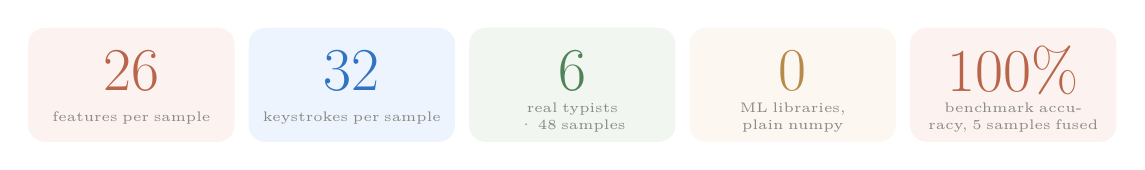
\begin{tikzpicture}
  \foreach \n/\l/\c [count=\i from 0] in
     {26/{features per sample}/terra,
      32/{keystrokes per sample}/sky,
      6/{real typists \textperiodcentered\ 48 samples}/sage,
      0/{ML libraries, plain numpy}/amber,
      100\%/{benchmark accuracy, 5 samples fused}/terra} {
    \node[stat=\c] (s\i) at (\i*2.8,0) {};
    \node[statnum=\c] at ($(s\i.center)+(0,0.18)$) {\n};
    \node[statlab] at ($(s\i.center)+(0,-0.42)$) {\l};
  }
\end{tikzpicture}
\end{frame}

% -----------------------------------------------------------------------------
\begin{frame}{Gamified enrollment: the test \emph{is} the sensor}
\begin{columns}[T,onlytextwidth]
\column{0.56\textwidth}
\begin{tikzpicture}[x=1cm,y=1cm]
  % --- the typing screen
  \fill[ink,rounded corners=8pt] (0,0) rectangle (7.7,-3.45);
  \foreach \c [count=\i] in {rose,amber,sage} \fill[\c] (0.05+\i*0.22,-0.2) circle (2.1pt);
  \node[fill=panel,rounded corners=6pt,font=\fontsize{5.4}{6}\selectfont,text=muted,inner xsep=6pt,inner ysep=3pt] at (3.85,-0.5)
    {@ punct\enspace \# num\enspace\textcolor{white!25!ink}{\textbar}\enspace
     \textcolor{terra}{\faIcon{stopwatch}\ time}\enspace words\enspace quote\enspace
     zen\enspace custom\enspace\textcolor{white!25!ink}{\textbar}\enspace
     15\enspace \textcolor{terra}{30}\enspace 60\enspace 120};
  \node[anchor=west,text=terra,font=\ttfamily\Large] at (0.3,-1.1) {23};
  \node[anchor=west,text=muted,font=\tiny] at (5.3,-1.1) {pace \faIcon{tachometer-alt}\ 80 wpm};
  \node[anchor=north west,text width=7.1cm,font=\ttfamily\footnotesize,align=left] at (0.28,-1.38)
    {\textcolor{cream}{the other way could peo}\textcolor{rose}{p}\textcolor{cream}{le}\caret\textcolor{muted}{\ find long day}\\[1pt]
     \textcolor{muted}{water sound \pacecaret word first write came}\\[1pt]
     \textcolor{muted!60!ink}{very thing our just name good line}};
  \node[text=muted!60!ink,font=\tiny] at (3.85,-3.2) {tab: new test \enspace\textbar\enspace esc: stop \enspace\textbar\enspace type to begin};

  % --- the results card
  \fill[ink,rounded corners=8pt] (0,-3.65) rectangle (7.7,-5.65);
  \node[anchor=north west,text=muted,font=\tiny] at (0.3,-3.78) {wpm};
  \node[anchor=north west,text=terra,font=\lightfont\fontsize{24}{24}\selectfont] at (0.25,-4.0) {72};
  \node[anchor=north west,text=muted,font=\tiny] at (1.55,-3.78) {acc};
  \node[anchor=north west,text=cream,font=\lightfont\fontsize{14}{14}\selectfont] at (1.5,-4.03) {96.4\%};
  \node[anchor=north west,text=cream!70,font=\tiny,align=left] at (0.3,-4.88) {+4 samples this session\\\textcolor{sage}{\faCheckCircle}\ 12 / 12 enrolled};
  \begin{scope}[shift={(3.55,-5.45)},xscale=0.93,yscale=0.95]
    \foreach \y in {0,0.5,1.0,1.5} \draw[white!14!ink,line width=0.4pt] (0,\y) -- (4.0,\y);
    \draw[sky,line width=0.9pt] plot coordinates {(0,0.55) (0.4,1.2) (0.8,0.95) (1.2,1.35) (1.6,0.7) (2.0,1.3) (2.4,1.0) (2.8,1.45) (3.2,0.8) (3.6,1.25) (4.0,1.1)};
    \draw[terra,line width=1.3pt] plot[smooth] coordinates {(0,0.45) (0.4,0.85) (0.8,0.98) (1.2,1.05) (1.6,1.02) (2.0,1.08) (2.4,1.07) (2.8,1.12) (3.2,1.1) (3.6,1.12) (4.0,1.13)};
    \foreach \p in {(1.6,0.7),(3.2,0.8)} \node[text=rose,font=\tiny\bfseries] at \p {\faTimes};
    \node[anchor=south east,font=\fontsize{5}{5}\selectfont,text=muted] at (4.0,1.5)
      {\textcolor{terra}{\rule{5pt}{1.5pt}} wpm \enspace \textcolor{sky}{\rule{5pt}{1.5pt}} raw \enspace \textcolor{rose}{\faTimes} error};
  \end{scope}
\end{tikzpicture}

\column{0.42\textwidth}
\small
\scriptsize
\begin{itemize}\setlength\itemsep{1.5pt}
\item \textbf{Monkeytype-style test}: \emph{time} (15--120\,s), \emph{words} (10--100), \emph{quote}, \emph{zen}, \emph{custom};
      punctuation \& numbers.
\item \textbf{Live feedback}: per-character colour, a gliding caret, a ghost \textbf{pace caret} (40--300\,wpm) to race.
\item \textbf{Score screen}: net wpm, accuracy, per-second raw-wpm chart with error marks.
\item \textbf{Visible progress}: “+4 samples added”; a milestone at 12 samples.
\end{itemize}
\vspace{1mm}
\begin{card}[terra]{\faLightbulb[regular]\ Why a game?}
\scriptsize Chasing a score, people type in their \emph{natural} rhythm. One 30\,s test yields \textbf{4 to 5 samples}.
\end{card}
\end{columns}
\end{frame}

% -----------------------------------------------------------------------------
\begin{frame}{Gamified identification: type until recognised}
\begin{columns}[c,onlytextwidth]
\column{0.47\textwidth}
\centering
\begin{tikzpicture}
  \node[st=terra] (T)  at (90:2.15)   {\textcolor{terra}{\faKeyboard}\ \textbf{Type a test}\\random words};
  \node[st=sky]   (C)  at (18:2.25)   {\textcolor{sky}{\faCut}\ \textbf{Cut}\\32-key samples};
  \node[st=amber] (M)  at (-54:2.2)   {\textcolor{amber!80!black}{\faCogs}\ \textbf{Match \& fuse}\\every template};
  \node[st=sage]  (Th) at (-126:2.2)  {\textcolor{sage}{\faBalanceScale}\ \textbf{Close enough?}\\\(d_{\min} \le \tau\)};
  \node[st=rose]  (U)  at (162:2.25)  {\textcolor{rose}{\faIcon{redo-alt}}\ \textbf{Not yet}\\fresh test dealt};
  \draw[lp=muted] (T) to[bend left=18] (C);
  \draw[lp=muted] (C) to[bend left=18] (M);
  \draw[lp=muted] (M) to[bend left=18] (Th);
  \draw[lp=rose]  (Th) to[bend left=18] node[left,font=\tiny,text=rose] {no} (U);
  \draw[lp=muted] (U) to[bend left=18] (T);
  \node[circle,fill=terra,text=white,minimum size=1.45cm,align=center,font=\tiny\bfseries,soft shadow] (W) at (0,-0.05)
     {{\Large\faTrophy}\\[1pt]RECOGNISED};
  \draw[lp=sage] (Th) -- node[pos=0.45,right,font=\tiny,text=sage] {yes} (W);
\end{tikzpicture}

\vspace{1mm}
{\scriptsize\color{muted}The name is then “typed out” letter by letter: a keystroke project answering in keystrokes.}

\column{0.5\textwidth}
\renewcommand\arraystretch{1.25}
\arrayrulecolor{line}
\scriptsize
\begin{tabular}{@{}>{\bfseries\raggedright\arraybackslash}p{2.25cm}>{\raggedright\arraybackslash}p{4.3cm}@{}}
\rowcolor{ink}\textcolor{cream}{Game mechanic} & \textcolor{cream}{\bfseries What it does for the biometric}\\
Timer \& wpm score  & keeps people at their natural, fluent pace \\ \midrule
Random word deals   & no memorised phrase \(\Rightarrow\) genuine free-text rhythm \\ \midrule
Pace caret          & a steady target, less hesitation noise \\ \midrule
Instant retry loop  & every miss adds samples to the next fused verdict \\ \midrule
Verdict reveal      & a pay-off moment; the \emph{margin} shows confidence \\ \midrule
Explain mode        & curiosity \(\rightarrow\) users see \emph{why} they were recognised \\
\end{tabular}
\end{columns}
\end{frame}

% -----------------------------------------------------------------------------
\begin{frame}{Limitations, honestly}
\begin{columns}[T,onlytextwidth]
\column{0.487\textwidth}
\begin{card}[rose]{\faDatabase\enspace Data}
\scriptsize
\badline{Only \textbf{6 real typists}, 48 samples, \textbf{one sitting} each.}
\badline{Real-data EER \textbf{19.0\,\%}, vs 5.9\,\% on the benchmark.}
\badline{New users shift everyone's normalisation.}
\end{card}
\begin{card}[amber]{\faUserClock\enspace Humans drift}
\scriptsize
\badline{Fatigue, mood, injury, new keyboards: rhythm drifts.}
\badline{Key-class features assume English with spaces.}
\badline{Needs \(\ge\)12 samples (\(\approx\)3 tests) per template.}
\end{card}
\column{0.487\textwidth}
\begin{card}[terradk]{\faIcon{shield-alt}\enspace Security}
\scriptsize
\badline{No liveness check: replays or trained mimics pass.}
\badline{Sensitive keystroke logs are stored as plain JSON.}
\badline{Impostor accepts: \(\approx\)7\,\% on the benchmark, 22\,\% on real data.}
\end{card}
\begin{card}[sky]{\faMicrochip\enspace Engineering}
\scriptsize
\badline{Tk timing: \(\approx\)5\,ms bias, \(\approx\)3\,ms animation jitter.}
\badline{Identifies typists; doesn't guard a real login yet.}
\badline{A desktop app, not a background OS-wide service.}
\end{card}
\end{columns}
\end{frame}

% =============================================================================
\renewcommand\secsub{From a key press to a verdict: capture, signals, spectrum, features, templates, decisions, and how we measured it.}
\section{Under the hood}
% =============================================================================

\begin{frame}{Architecture: two halves that never mix}
\centering
\begin{tikzpicture}[node distance=4pt, chip/.append style={font=\fontsize{6.7}{9}\selectfont, inner xsep=2.8pt, inner ysep=5pt, minimum height=0.95cm}]
  % ---------------- UI
  \node[anchor=west,font=\small\bfseries,text=sky] (uit) at (0,0)
    {\faDesktop\ keyloggd.ui \textmd{\color{muted}\scriptsize\enspace Tkinter front end \textperiodcentered\ standard library only \textperiodcentered\ owns no maths}};
  \node[chip=sky,below right=9pt and 0pt of uit.south west] (u1) {\ttfamily app\\\tiny\color{muted}3 views, worker thread};
  \node[chip=sky,right=of u1] (u2) {\ttfamily typing\_test\\\tiny\color{muted}Monkeytype test};
  \node[chip=sky,right=of u2] (u3) {\ttfamily explain\\\tiny\color{muted}6-phase walk-through};
  \node[chip=sky,right=of u3] (u4) {\ttfamily charts\\\tiny\color{muted}canvas plots};
  \node[chip=sky,right=of u4] (u5) {\ttfamily splash\\\tiny\color{muted}warm start};
  \node[chip=sky,right=of u5] (u6) {\ttfamily anim\\\tiny\color{muted}60\,fps tweens};
  \node[chip=sky,right=of u6] (u7) {\ttfamily theme\\\tiny\color{muted}palette, fonts};
  \begin{scope}[on background layer]
    \node[fit=(uit)(u1)(u7),rounded corners=7pt,fill=sky!7,draw=sky!45,inner xsep=7pt,inner ysep=8pt,line width=0.7pt] (UI) {};
  \end{scope}

  % ---------------- pipeline
  \node[anchor=west,font=\small\bfseries,text=terradk] (pt) at (0,-2.67)
    {\faProjectDiagram\ keyloggd.pipeline \textmd{\color{muted}\scriptsize\enspace signal processing \textperiodcentered\ numpy only \textperiodcentered\ no Tk import}};
  \node[chip=terra,below right=9pt and 0pt of pt.south west] (p1) {\ttfamily samples\\\tiny\color{muted}32-key windows};
  \node[chip=terra,right=of p1] (p2) {\ttfamily signal\_construction\\\tiny\color{muted}dwell / flight};
  \node[chip=terra,right=of p2] (p3) {\ttfamily timing\_features\\\tiny\color{muted}26-D vector};
  \node[chip=terra,right=of p3] (p4) {\ttfamily fft\_features\\\tiny\color{muted}spectrum};
  \node[chip=terra,right=of p4] (p5) {\ttfamily denoise\\\tiny\color{muted}low-pass};
  \node[chip=terra,right=of p5] (p6) {\ttfamily classifier\\\tiny\color{muted}templates, EER};
  \node[chip=terra,right=of p6] (p7) {\ttfamily identify\_sample\\\tiny\color{muted}fuse, verdict};
  \begin{scope}[on background layer]
    \node[fit=(pt)(p1)(p7),rounded corners=7pt,fill=terra!7,draw=terra!45,inner xsep=7pt,inner ysep=8pt,line width=0.7pt] (PL) {};
  \end{scope}

  % ---------------- tools + data
  \node[chip=amber,anchor=north west,text width=8.1cm,align=left,inner sep=5pt,minimum height=0pt,font=\scriptsize] (tools) at ($(PL.south west)+(0,-0.32)$)
    {\textbf{\faFlask\ tools/}\quad{\ttfamily\fontsize{6.4}{8}\selectfont synthetic\_data\_generator \textperiodcentered\ benchmark\_inference}\\
     {\tiny\color{muted}simulated typists with rollover \& pauses; the cross-phrase benchmark}};
  \node[cylinder,shape border rotate=90,aspect=0.18,draw=sage!70,fill=sage!10,minimum width=1.45cm,minimum height=0.9cm,
        anchor=north east,font=\tiny,align=center,line width=0.7pt] (db) at ($(PL.south east)+(-0.2,-0.35)$)
    {\faUsers\\ \texttt{<user>.json}\\ \(\times 6\)};
  \node[anchor=east,font=\scriptsize,text width=3.4cm,align=right,text=muted] at ($(db.west)+(-0.2,0)$)
    {\texttt{data/synthetic/}\\one JSON file per typist};

  \draw[flow,sky] (UI.south -| u3.south) -- (PL.north -| u3.south);
  \draw[flow] (tools.north -| p2.south) -- (PL.south -| p2.south);
  \draw[flow,sage,{Stealth[round]}-{Stealth[round]}] (db.north) -- (PL.south -| db.north);
\end{tikzpicture}
\end{frame}

% -----------------------------------------------------------------------------
\begin{frame}{End-to-end data flow}
\centering
\begin{tikzpicture}
  \def\dx{3.5}
  % row 1  (left -> right)
  \node[stage=terra] (s1) at (0,0)      {\faKeyboard\ \textbf{keydown / keyup}\\Tk key events};
  \node[stage=terra] (s2) at (\dx,0)    {\texttt{perf\_counter()}\\\(\mu\)s timestamps, held-key filter};
  \node[stage=terra] (s3) at (2*\dx,0)  {\textbf{raw event stream}\\\texttt{\{key, type, t\}}};
  \node[stage=terra] (s4) at (3*\dx,0)  {\texttt{split\_into\_samples}\\32 keys \textperiodcentered\ tail \(<\)16 dropped};
  % row 2  (right -> left)
  \node[stage=sky] (s5) at (3*\dx,-1.75) {\texttt{events\_to\_signal}\\\(d[n]\), \(f[n]\)};
  \node[stage=sky] (s6) at (2*\dx,-1.75) {\texttt{feature\_vector}\\26 robust statistics};
  \node[stage=amber] (s7) at (\dx,-1.75) {\texttt{ZScoreScaler}\\fit on enrolled data only};
  \node[stage=amber] (s8) at (0,-1.75)   {\texttt{build\_templates}\\mean + spread per user};
  % row 3  (left -> right)
  \node[stage=sage] (s9)  at (0,-3.5)      {\texttt{template\_distance}\\scaled Manhattan};
  \node[stage=sage] (s10) at (\dx,-3.5)    {\texttt{knn\_predict}\\\(k{=}3\), \(1/d\) weights};
  \node[stage=sage] (s11) at (2*\dx,-3.5)  {\texttt{fuse}\\mean distance over the run};
  \node[stage=sage,fill=sage!25,line width=1.1pt] (s12) at (3*\dx,-3.5) {\textbf{verdict}\\name if \(d \le \tau\), else \textsc{unrecognized}};

  \foreach \a/\b in {s1/s2,s2/s3,s3/s4,s5/s6,s6/s7,s7/s8,s9/s10,s10/s11,s11/s12} \draw[flow] (\a) -- (\b);
  \draw[flow] (s4) -- (s5);
  \draw[flow] (s8) -- (s9);
  \foreach \s [count=\i] in {s1,s2,s3,s4,s5,s6,s7,s8,s9,s10,s11,s12}
    \node[n=ink] at (\s.north west) {\i};

  % legend
  \node[anchor=north,font=\scriptsize] at (1.5*\dx,-4.4)
    {\swatch{terra} capture \qquad \swatch{sky} signal \& features \qquad \swatch{amber} model \qquad \swatch{sage} decision
     \qquad \textcolor{muted}{every box is a real function}};
\end{tikzpicture}
\end{frame}

% -----------------------------------------------------------------------------
\begin{frame}[fragile]{Step 1 \textperiodcentered\ Capture: timestamping every key}
\begin{columns}[T,onlytextwidth]
\column{0.51\textwidth}
\small
\begin{itemize}\setlength\itemsep{2pt}
\item Tk \code{<KeyPress>} / \code{<KeyRelease>} are routed into the typing test.
\item \(t = \) \code{time.perf\_counter()} \(-\) session start, rounded to \textbf{1\,\(\mu\)s} (6 decimals).
\item A \textbf{held-key set} drops OS auto-repeat: a second keydown with no keyup between would pair the wrong two timestamps.
\item Only printable keys and space are recorded. \textbf{Backspace} edits the screen, not the signal;
      \textbf{Tab} deals a new test, \textbf{Esc} stops.
\item The first keystroke \emph{settles} any running animation, so it can't delay a later timestamp.
\end{itemize}
\column{0.46\textwidth}
\begin{tcolorbox}[enhanced,colback=ink,colframe=ink,arc=6pt,left=2pt,right=2pt,top=6pt,bottom=6pt,
  title={\faFileCode[regular]\ \ttfamily data/synthetic/swayam.json},fonttitle=\scriptsize,coltitle=muted,colbacktitle=ink,
  titlerule=0.4pt,colframe=ink,fuzzy shadow={0.4pt}{-0.9pt}{0pt}{0.35pt}{black!20}]
\begin{lstlisting}[style=json]
{ "user_id": "swayam",
  "phrase": "free text (typing test)",
  "samples": [
   { "events": [
     {"key": "o", "type": "down", "t": 0.0},
     {"key": "o", "type": "up", "t": 0.069164},
     {"key": "t", "type": "down", "t": 0.197467},
     {"key": "t", "type": "up", "t": 0.269857},
     ... ],
     "phrase": "other me yopur ur ferom ...",
     "captured_at": "2026-09-12T23:26:00" },
   ... ] }
\end{lstlisting}
\end{tcolorbox}
{\scriptsize\color{muted}One schema everywhere: the synthetic generator, the typing test and the phrase widget all write it.}
\end{columns}
\end{frame}

% -----------------------------------------------------------------------------
\begin{frame}{Step 2 \textperiodcentered\ Dwell, flight and rollover}
\begin{columns}[T,onlytextwidth]
\column{0.64\textwidth}
\begin{tikzpicture}[x=13.8cm,y=1cm]
  \foreach \k/\y in {o/2.4,t/1.9,h/1.4,e/0.9,r/0.4} {\node[font=\ttfamily\small,text=muted,anchor=east] at (-0.005,\y) {\k}; \draw[line] (0,\y) -- (0.64,\y);}
  \draw[dkey] (0.000,2.25) rectangle (0.069,2.55);
  \draw[dkey] (0.197,1.75) rectangle (0.270,2.05);
  \draw[dkey] (0.358,1.25) rectangle (0.429,1.55);
  \draw[dkey] (0.454,0.75) rectangle (0.549,1.05);
  \draw[dkey] (0.518,0.25) rectangle (0.621,0.55);
  \foreach \x/\y/\v in {0.0345/2.4/69, 0.2335/1.9/72, 0.3935/1.4/72, 0.5015/0.9/94, 0.5695/0.4/103}
    \node[font=\tiny\bfseries,text=white] at (\x,\y) {\v};
  % flights
  \foreach \a/\b/\y/\v in {0.069/0.197/2.1/128, 0.270/0.358/1.6/88, 0.429/0.454/1.1/25} {
    \draw[sky,densely dotted] (\a,\y+0.15) -- (\a,\y);
    \draw[sky,line width=0.9pt,-{Stealth[length=3.5pt]}] (\a,\y) -- (\b,\y);
    \node[font=\tiny,text=sky,below] at ({(\a+\b)/2},\y) {\v};
  }
  \fill[rose,opacity=0.22] (0.518,0.25) rectangle (0.549,1.05);
  \draw[rose,line width=0.9pt,{Stealth[length=3.5pt]}-{Stealth[length=3.5pt]}] (0.518,0.12) -- (0.549,0.12);
  \node[font=\tiny\bfseries,text=rose!85!black,anchor=north] at (0.5335,0.1) {\(-31\) ms rollover};
  % axis
  \draw[muted] (0,-0.35) -- (0.64,-0.35);
  \foreach \t in {0,0.1,...,0.61} \draw[muted] (\t,-0.35) -- ++(0,-0.07) node[below,font=\tiny,text=muted] {\pgfmathprintnumber[fixed,precision=1]{\t}};
  \node[font=\tiny,text=muted,anchor=west] at (0.645,-0.5) {s};
  \node[font=\tiny,text=muted,anchor=west] at (0,2.85) {\swatch{terra} dwell (ms) \quad \textcolor{sky}{\faLongArrowAltRight} flight (ms) \quad (the first five keys of a real sample)};
\end{tikzpicture}

\column{0.34\textwidth}
\begin{card}[terra]{Two discrete signals}
\[
\begin{aligned}
d[n] &= t^{\uparrow}_{n} - t^{\downarrow}_{n}\\
f[n] &= t^{\downarrow}_{n+1} - t^{\uparrow}_{n}
\end{aligned}
\]
\scriptsize \(N\) keystrokes \(\Rightarrow\) \(N\) dwells, \(N{-}1\) flights.\\[2pt]
\(f[n] < 0\) \(\iff\) \textbf{rollover}: the next key went down first.
\end{card}
\end{columns}

\vspace{2mm}
\begin{tcolorbox}[enhanced,colback=sky!6,colframe=sky!35,boxrule=0.5pt,arc=4pt,left=8pt,right=8pt,top=2pt,bottom=2pt]
\scriptsize\textbf{\color{sky}Signal view.} The true process is an impulse train \(x(t)=\sum_i \delta(t-t_i)\) at the key-down times.
\(d[n]\) and \(f[n]\) sample it \emph{at the events} rather than at fixed time steps, and everything downstream treats them as discrete-time signals.
\end{tcolorbox}
\end{frame}

% -----------------------------------------------------------------------------
\begin{frame}{Step 3 \textperiodcentered\ Slicing one long run into samples}
\centering
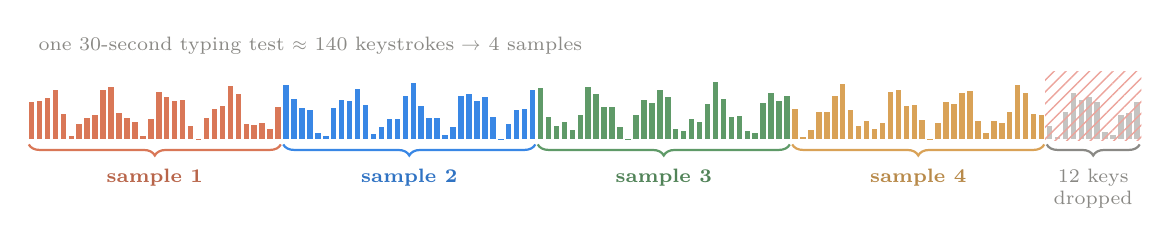
\begin{tikzpicture}[x=1cm,y=1cm]
  % 140 keystrokes, cut into 32-key windows
  \foreach \i in {0,...,139} {
    \pgfmathtruncatemacro\w{int(\i/32)}
    \ifnum\w=0 \def\c{terra}\fi \ifnum\w=1 \def\c{sky}\fi \ifnum\w=2 \def\c{sage}\fi
    \ifnum\w=3 \def\c{amber}\fi \ifnum\w=4 \def\c{muted!50}\fi
    \pgfmathsetmacro\h{0.35+0.25*sin(\i*47)+0.12*cos(\i*113)}
    \fill[\c] (\i*0.101,0) rectangle ++(0.07,\h);
  }
  \foreach \s/\e/\l/\c in {0/31/{sample 1}/terra, 32/63/{sample 2}/sky, 64/95/{sample 3}/sage, 96/127/{sample 4}/amber} {
    \draw[decorate,decoration={brace,mirror,amplitude=4pt,raise=2pt},\c,line width=0.8pt] (\s*0.101,0) -- (\e*0.101+0.07,0)
      node[midway,below=7pt,font=\scriptsize\bfseries,text=\c!85!black] {\l};
  }
  \draw[decorate,decoration={brace,mirror,amplitude=4pt,raise=2pt},muted,line width=0.8pt] (128*0.101,0) -- (139*0.101+0.07,0)
      node[midway,below=7pt,font=\scriptsize,text=muted,align=center] {12 keys\\dropped};
  \fill[pattern={Lines[angle=45,distance=3pt,line width=0.5pt]},pattern color=rose!60] (128*0.101-0.02,-0.02) rectangle (139*0.101+0.09,0.85);
  \node[anchor=south west,font=\scriptsize,text=muted] at (0,0.95) {one 30-second typing test \(\approx\) 140 keystrokes \(\rightarrow\) 4 samples};
\end{tikzpicture}

\vspace{3mm}
\begin{columns}[T,onlytextwidth]
\column{0.32\textwidth}
\begin{card}[terra]{\faLink\ Pairing}
\scriptsize Each \emph{down} is matched to the next \emph{up} of the same key, so overlapping keys (rollover)
pair correctly. A down with no up is dropped, never guessed.
\end{card}
\column{0.32\textwidth}
\begin{card}[sky]{\faCut\ Windows of 32}
\scriptsize Enough keys for a stable median / IQR, yet 4--5 samples per test for the fused verdict.
A tail under \textbf{16} keys (\code{MIN\_KEYS}) describes noise more than the typist, so it is dropped.
\end{card}
\column{0.32\textwidth}
\begin{card}[sage]{\faRedo\ Rebasing}
\scriptsize Each window's times are shifted so its first keydown is \(t{=}0\). Only differences are ever used, so no
feature changes; every sample just reads like any other.
\end{card}
\end{columns}
\end{frame}

% -----------------------------------------------------------------------------
\begin{frame}{A real sample, as the pipeline sees it}
\centering
\begin{tikzpicture}
\begin{axis}[kl, width=15cm, height=5.4cm, ybar, bar width=3.3pt,
    ymin=-140, ymax=320, xmin=-0.8, xmax=31.8, enlarge x limits=false,
    ymajorgrids, ylabel={milliseconds},
    xtick={0,...,31},
    xticklabels={o,t,h,e,r,\textperiodcentered,m,e,\textperiodcentered,y,o,p,u,r,\textperiodcentered,u,r,\textperiodcentered,f,e,r,o,m,\textperiodcentered,o,t,h,e,r,\textperiodcentered,s,o},
    xticklabel style={font=\ttfamily\scriptsize,text=ink}, major x tick style={draw=none},
    clip mode=individual, legend style={at={(0.01,0.98)},anchor=north west}, legend columns=2]
  \addplot[fill=terra, draw=none, bar shift=0pt] coordinates {(0,69) (1,72) (2,72) (3,94) (4,103) (5,55) (6,97) (7,96) (8,70) (9,79) (10,125) (11,92) (12,112) (13,87) (14,54) (15,72) (16,78) (17,55) (18,110) (19,94) (20,94) (21,136) (22,80) (23,96) (24,87) (25,63) (26,87) (27,103) (28,89) (29,53) (30,111) (31,79)};
  \addplot[fill=sky, draw=none, bar shift=0pt] coordinates {(0.5,128) (1.5,88) (2.5,25) (3.5,-31) (4.5,49) (5.5,113) (6.5,39) (7.5,50) (8.5,266) (9.5,2) (10.5,-115) (11.5,-9) (12.5,80) (13.5,82) (14.5,1370) (15.5,57) (16.5,89) (17.5,201) (18.5,-22) (19.5,282) (20.5,33) (21.5,-40) (22.5,80) (23.5,161) (24.5,162) (25.5,88) (26.5,1) (27.5,-32) (28.5,1) (29.5,90) (30.5,-55)};
  \legend{dwell \(d[n]\), flight \(f[n]\)}
  \draw[muted] (axis cs:-0.8,0) -- (axis cs:31.8,0);
  \node[pill=ink,anchor=west] at (axis cs:15.1,292) {\faHourglassHalf\ 1\,370\,ms think-pause (clipped)};
  \draw[ink,-{Stealth[length=4pt]}] (axis cs:15.1,292) -- (axis cs:14.75,305);
  \node[pill=rose,anchor=north] at (axis cs:10.5,-120) {rollover \(-115\) ms};
\end{axis}
\end{tikzpicture}

\vspace{1mm}
\small Typed: \texttt{"other me yopur ur ferom other so"}, typos and all. \textcolor{muted}{The features never read the text,
only the timing; free text is the point.} One pause is \(\approx\)20\(\times\) a normal flight: anything built on a mean or a total would be ruled by it.
\end{frame}

% -----------------------------------------------------------------------------
\begin{frame}{What our six real typists look like}
\begin{columns}[c,onlytextwidth]
\column{0.5\textwidth}
\scriptsize
\renewcommand\arraystretch{1.25}
\setlength\tabcolsep{4.5pt}
\arrayrulecolor{line}
\begin{tabular}{@{}l r r r r l@{}}
\rowcolor{ink}
\textcolor{cream}{\bfseries user} & \textcolor{cream}{samples} & \textcolor{cream}{keys} & \textcolor{cream}{\(\tilde d\) ms} & \textcolor{cream}{\(\tilde f\) ms} & \textcolor{cream}{rollover}\\
\texttt{ahnaf}  &  7 & 219 & 101 &   2 & \rbar{35.8}\\ \midrule
\texttt{arghya} &  8 & 232 &  97 & 103 & \rbar{0.0}\\ \midrule
\texttt{nafis}  &  7 & 224 &  82 &  19 & \rbar{25.3}\\ \midrule
\texttt{newbie} &  3 &  88 &  80 & 208 & \rbar{7.1}\\ \midrule
\texttt{swayam} & 16 & 492 &  88 &  73 & \rbar{15.3}\\ \midrule
\texttt{tahmid} &  7 & 214 &  83 & 109 & \rbar{8.2}\\ \midrule
\textbf{total}  & \textbf{48} & \textbf{1469} & & & \\
\end{tabular}

\vspace{1mm}
{\scriptsize\color{muted}\(\tilde d, \tilde f\) = median dwell / flight over all of a user's keystrokes. All captured through the typing test.}

\column{0.47\textwidth}
\raggedleft
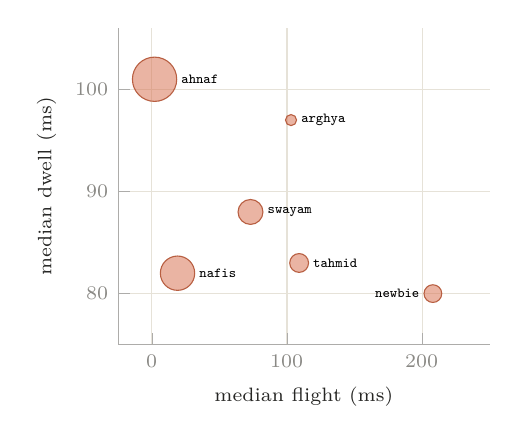
\begin{tikzpicture}
\begin{axis}[kl, width=6.3cm, height=5.6cm, xmin=-25, xmax=250, ymin=75, ymax=106,
   xlabel={median flight (ms)}, ylabel={median dwell (ms)}, xmajorgrids, ymajorgrids, clip=false]
  \foreach \x/\y/\s/\n/\a in {2/101/8.0/ahnaf/west, 103/97/2.0/arghya/west,
      19/82/6.2/nafis/west, 208/80/3.2/newbie/east, 73/88/4.5/swayam/west, 109/83/3.4/tahmid/west} {
    \edef\temp{\noexpand\addplot[only marks, mark=*, mark size=\s pt, mark options={fill=terra, fill opacity=0.55, draw=terradk}] coordinates {(\x,\y)};
      \noexpand\node[font=\noexpand\tiny\noexpand\ttfamily, anchor=\a, inner sep=\s pt+1.5pt] at (axis cs:\x,\y) {\n};}
    \temp
  }
\end{axis}
\end{tikzpicture}

{\scriptsize\color{muted}bubble size = rollover rate. \texttt{ahnaf} and \texttt{nafis} roll over constantly; \texttt{arghya} never does.}
\end{columns}
\end{frame}

% -----------------------------------------------------------------------------
\begin{frame}{Step 4a \textperiodcentered\ The frequency-domain view of rhythm}
\begin{columns}[c,onlytextwidth]
\column{0.58\textwidth}
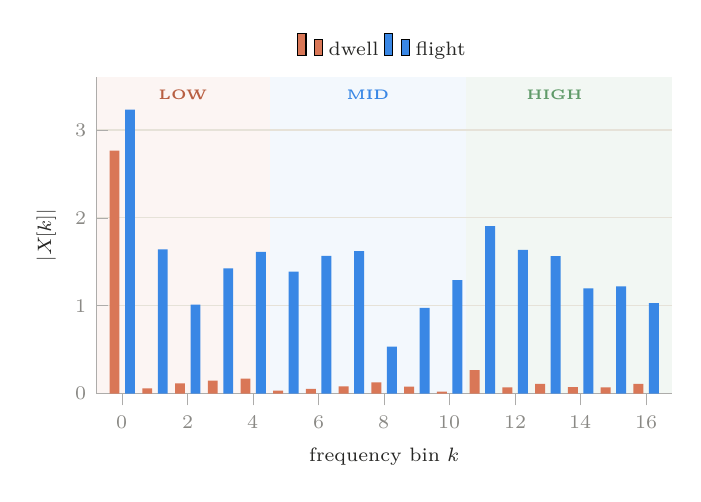
\begin{tikzpicture}
\begin{axis}[kl, set layers, ybar, bar width=3.6pt, width=8.9cm, height=5.6cm,
   xmin=-0.8, xmax=16.8, ymin=0, ymax=3.6, enlarge x limits=false,
   xlabel={frequency bin \(k\)}, ylabel={\(|X[k]|\)}, xtick={0,2,...,16}, ymajorgrids,
   legend style={at={(0.5,1.02)},anchor=south}, legend columns=2]
  \begin{pgfonlayer}{axis background}
    \fill[terra!7] (axis cs:-0.8,0) rectangle (axis cs:4.5,3.6);
    \fill[sky!6]   (axis cs:4.5,0)  rectangle (axis cs:10.5,3.6);
    \fill[sage!8]  (axis cs:10.5,0) rectangle (axis cs:16.8,3.6);
  \end{pgfonlayer}
  \addplot[fill=terra, draw=none] coordinates {(0,2.766) (1,0.060) (2,0.117) (3,0.147) (4,0.172) (5,0.035) (6,0.053) (7,0.082) (8,0.129) (9,0.081) (10,0.023) (11,0.266) (12,0.070) (13,0.110) (14,0.074) (15,0.070) (16,0.111)};
  \addplot[fill=sky, draw=none] coordinates {(0,3.231) (1,1.641) (2,1.013) (3,1.425) (4,1.612) (5,1.388) (6,1.566) (7,1.621) (8,0.536) (9,0.975) (10,1.290) (11,1.907) (12,1.636) (13,1.563) (14,1.197) (15,1.219) (16,1.029)};
  \legend{dwell, flight}
  \node[font=\tiny\bfseries,text=terradk] at (axis cs:1.85,3.4) {LOW};
  \node[font=\tiny\bfseries,text=sky]     at (axis cs:7.5,3.4) {MID};
  \node[font=\tiny\bfseries,text=sage]    at (axis cs:13.2,3.4) {HIGH};
\end{axis}
\end{tikzpicture}
{\scriptsize\color{muted}\ Same real sample. Input is real, so 17 of the 32 bins are unique.}

\column{0.39\textwidth}
\begin{card}[terra]{The transform}
\centering\(X[k] = \sum_{n=0}^{N-1} x[n]\, e^{-j 2\pi k n / N}\)\par\vspace{3pt}
\raggedright\scriptsize \(N = 32\). First bring \(x\) to that length: \textbf{zero-pad}, or \textbf{resample} by linear interpolation for free text.
\end{card}
\begin{card}[sky]{5 numbers per stream}
\scriptsize
\(\text{centroid} = \sum_k k|X_k| / \sum_k |X_k|\)\\[2pt]
\(E_{\text{band}} = \sum_{\text{band}} |X_k|^2 / \sum_k |X_k|^2\)\ \ (low, mid, high)\\[2pt]
+ total energy; with mean/std of \(d, f\): the original \textbf{14-D} vector.
\end{card}
\end{columns}
\end{frame}

% -----------------------------------------------------------------------------
\begin{frame}{Step 4b \textperiodcentered\ Denoising with an FFT low-pass filter}
\centering
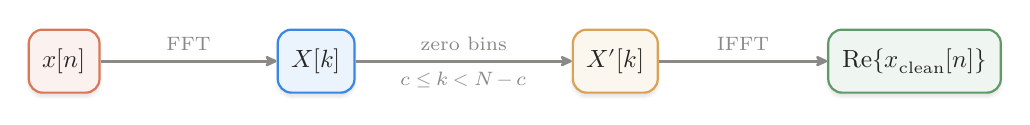
\begin{tikzpicture}
  \node[sig=terra] (a) at (0,0) {\(x[n]\)};
  \node[sig=sky]   (b) at (3.2,0) {\(X[k]\)};
  \node[sig=amber] (c) at (7.0,0) {\(X'[k]\)};
  \node[sig=sage]  (d) at (10.8,0) {\(\mathrm{Re}\{x_{\text{clean}}[n]\}\)};
  \draw[flow] (a) -- node[above,font=\scriptsize] {FFT} (b);
  \draw[flow] (b) -- node[above,font=\scriptsize,align=center] {zero bins} node[below,font=\scriptsize] {\(c \le k < N-c\)} (c);
  \draw[flow] (c) -- node[above,font=\scriptsize] {IFFT} (d);
\end{tikzpicture}

\vspace{3mm}
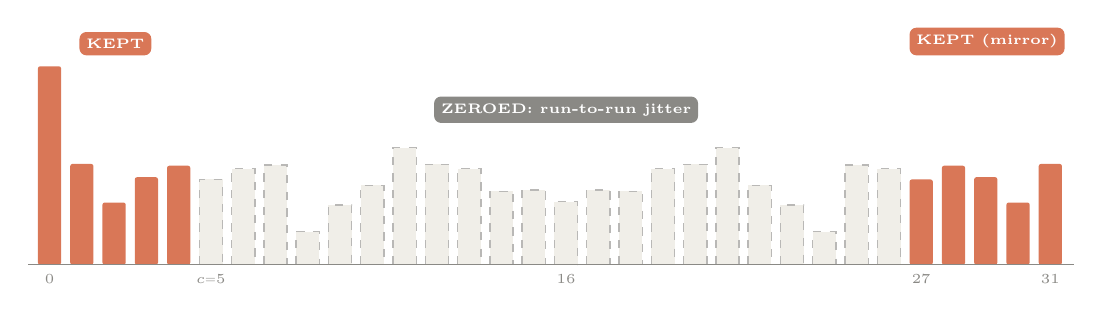
\begin{tikzpicture}[x=0.41cm,y=0.78cm]
  \foreach \v [count=\k from 0] in {3.231,1.641,1.013,1.425,1.612,1.388,1.566,1.621,0.536,0.975,1.290,1.907,1.636,1.563,1.197,1.219,1.029,1.219,1.197,1.563,1.636,1.907,1.290,0.975,0.536,1.621,1.566,1.388,1.612,1.425,1.013,1.641} {
    \ifnum\k<5 \fill[terra,rounded corners=0.8pt] (\k,0) rectangle ++(0.72,\v);
    \else\ifnum\k>26 \fill[terra,rounded corners=0.8pt] (\k,0) rectangle ++(0.72,\v);
    \else \draw[muted!60,dashed,line width=0.5pt,fill=line!60] (\k,0) rectangle ++(0.72,\v);
    \fi\fi
    \ifnum\k=0 \node[below,font=\tiny,text=muted] at (\k+0.36,0) {0};\fi
    \ifnum\k=5 \node[below,font=\tiny,text=muted] at (\k+0.36,0) {\(c{=}5\)};\fi
    \ifnum\k=16 \node[below,font=\tiny,text=muted] at (\k+0.36,0) {16};\fi
    \ifnum\k=27 \node[below,font=\tiny,text=muted] at (\k+0.36,0) {27};\fi
    \ifnum\k=31 \node[below,font=\tiny,text=muted] at (\k+0.36,0) {31};\fi
  }
  \draw[muted] (-0.3,0) -- (32.1,0);
  \node[pill=terra,anchor=south] at (2.4,3.4) {KEPT};
  \node[pill=muted,anchor=south] at (16.36,2.3) {ZEROED: run-to-run jitter};
  \node[pill=terra,anchor=south] at (29.4,3.4) {KEPT (mirror)};
\end{tikzpicture}

\vspace{2mm}
\small \(c = \max\!\big(1, \lfloor \tfrac{N}{2}\cdot 0.35 \rfloor\big) = 5\): keep the lowest 35\,\% of the half-spectrum, zeroing
\emph{both} sides so conjugate symmetry holds and the inverse FFT stays real.
\textcolor{muted}{High frequencies \(\approx\) jitter, low frequencies \(\approx\) the stable rhythm.}
\end{frame}

% -----------------------------------------------------------------------------
\begin{frame}{Step 4c \textperiodcentered\ Why the spectrum lost}
\begin{columns}[c,onlytextwidth]
\column{0.42\textwidth}
\begin{card}[rose]{\faIcon{compress-arrows-alt}\ 1 \enspace Too few points}
\scriptsize 20--40 keys per sample: 17 bins from \(\sim\)30 noisy points. Three band ratios keep the noise, lose the structure.
\end{card}
\begin{card}[rose]{\faRulerHorizontal\ 2 \enspace Length leaks in}
\scriptsize Zero-padding makes the spectrum depend on \emph{how long the text was}: fatal on free text.
\end{card}
\begin{card}[rose]{\faHourglassHalf\ 3 \enspace One pause rules}
\scriptsize A 1.3\,s gap \(\approx\)20\(\times\) a 70\,ms one: total energy is decided by one hesitation.
\end{card}

\column{0.55\textwidth}
\centering
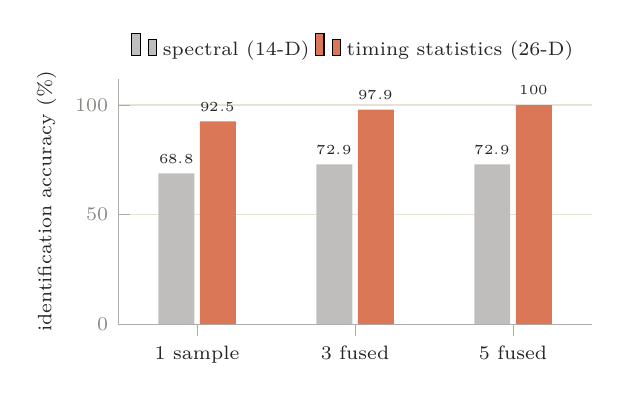
\begin{tikzpicture}
\begin{axis}[kl, ybar, bar width=13pt, width=7.6cm, height=4.7cm, ymin=0, ymax=112,
    symbolic x coords={1 sample, 3 fused, 5 fused}, xtick=data, ymajorgrids,
    ylabel={identification accuracy (\%)}, enlarge x limits=0.25,
    nodes near coords, every node near coord/.append style={font=\tiny, text=ink},
    legend style={at={(0.5,1.03)},anchor=south}, legend columns=2, x tick label style={font=\scriptsize,text=ink}]
  \addplot[fill=muted!55, draw=none] coordinates {(1 sample,68.8) (3 fused,72.9) (5 fused,72.9)};
  \addplot[fill=terra, draw=none] coordinates {(1 sample,92.5) (3 fused,97.9) (5 fused,100)};
  \legend{spectral (14-D)\quad, timing statistics (26-D)}
\end{axis}
\end{tikzpicture}

\small Verification EER: \textbf{18.72\,\% \(\rightarrow\) 5.89\,\%}\\[2pt]
{\scriptsize\color{muted}Cross-phrase benchmark. Spectral features added back on top (raw, compressed, 2/4/6 bins) cost accuracy every time, so
the spectrum stays for \emph{denoise} and \emph{explain}, not the decision.}
\end{columns}
\end{frame}

% -----------------------------------------------------------------------------
\begin{frame}{Step 5a \textperiodcentered\ Taming pauses and rollover with \(\operatorname{asinh}\)}
\begin{columns}[c,onlytextwidth]
\column{0.55\textwidth}
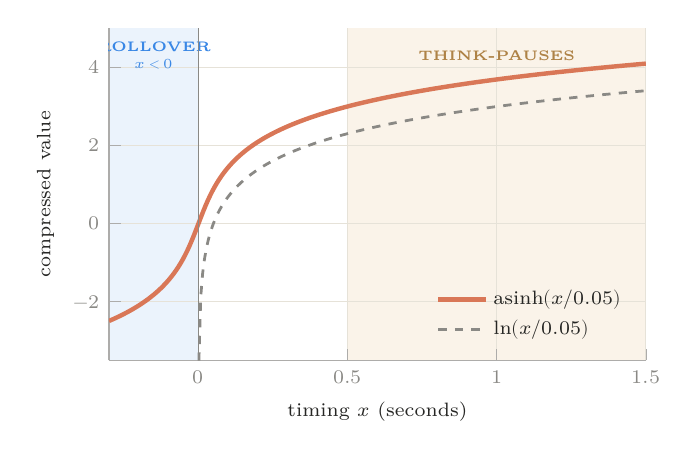
\begin{tikzpicture}
\begin{axis}[kl, set layers, width=8.4cm, height=5.8cm, xmin=-0.3, xmax=1.5, ymin=-3.5, ymax=5,
    xlabel={timing \(x\) (seconds)}, ylabel={compressed value}, samples=240, ymajorgrids, xmajorgrids,
    legend style={at={(0.98,0.03)},anchor=south east}]
  \begin{pgfonlayer}{axis background}
    \fill[sky!10] (axis cs:-0.3,-3.5) rectangle (axis cs:0,5);
    \fill[amber!13] (axis cs:0.5,-3.5) rectangle (axis cs:1.5,5);
  \end{pgfonlayer}
  \addplot[terra, line width=1.6pt, domain=-0.3:1.5] {ln(x/0.05 + sqrt((x/0.05)^2+1))};
  \addplot[muted, dashed, line width=1pt, domain=0.0015:1.5] {ln(x/0.05)};
  \legend{\(\operatorname{asinh}(x/0.05)\), \(\ln(x/0.05)\)}
  \node[font=\tiny\bfseries,text=sky,align=center] at (axis cs:-0.15,4.3) {ROLLOVER\\\(x<0\)};
  \node[font=\tiny\bfseries,text=amber!80!black,align=center] at (axis cs:1.0,4.3) {THINK-PAUSES};
  \draw[muted] (axis cs:0,-3.5) -- (axis cs:0,5);
\end{axis}
\end{tikzpicture}

\column{0.42\textwidth}
\centering\(\displaystyle a(x) = \operatorname{asinh}\!\left(\frac{x}{s}\right), \qquad s = 0.05\text{ s}\)\par\vspace{2mm}\raggedright
\small
\begin{itemize}\setlength\itemsep{1.5pt}
\item \textbf{Linear near zero}: ordinary flights (\(\sim\)50\,ms \(= s\)) keep their resolution.
\item \textbf{Logarithmic in the tails}: a 1.3\,s pause is squashed like a log.
\item \textbf{Sign-aware}: rollover keeps its sign. \(\ln\) can't take \(x \le 0\); clamping would send
      \emph{every} rollover to one huge negative value.
\item Ratios as \(a(x)-a(y)\): a log-ratio normally, still finite as \(y\to 0\).
\end{itemize}
\end{columns}
\end{frame}

% -----------------------------------------------------------------------------
\begin{frame}{Step 5b \textperiodcentered\ The 26-dimensional feature vector}
\centering
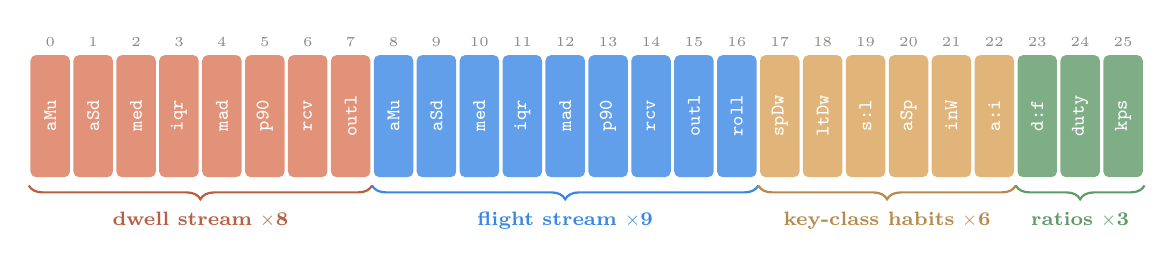
\begin{tikzpicture}[x=0.545cm,y=1cm]
  \foreach \c/\col [count=\i from 0] in {aMu/terra,aSd/terra,med/terra,iqr/terra,mad/terra,p90/terra,rcv/terra,outl/terra,
      aMu/sky,aSd/sky,med/sky,iqr/sky,mad/sky,p90/sky,rcv/sky,outl/sky,roll/sky,
      spDw/amber,ltDw/amber,s:l/amber,aSp/amber,inW/amber,a:i/amber,
      d:f/sage,duty/sage,kps/sage} {
    \fill[\col!80,rounded corners=2pt] (\i+0.04,0) rectangle (\i+0.96,1.55);
    \node[rotate=90,font=\ttfamily\scriptsize,text=white] at (\i+0.5,0.78) {\c};
    \node[font=\fontsize{5}{5}\selectfont,text=muted] at (\i+0.5,1.72) {\i};
  }
  \draw[decorate,decoration={brace,mirror,amplitude=5pt,raise=3pt},terradk,line width=0.8pt] (0,0) -- (8,0) node[midway,below=9pt,font=\scriptsize\bfseries,text=terradk] {dwell stream \(\times\)8};
  \draw[decorate,decoration={brace,mirror,amplitude=5pt,raise=3pt},sky,line width=0.8pt] (8,0) -- (17,0) node[midway,below=9pt,font=\scriptsize\bfseries,text=sky] {flight stream \(\times\)9};
  \draw[decorate,decoration={brace,mirror,amplitude=5pt,raise=3pt},amber!85!black,line width=0.8pt] (17,0) -- (23,0) node[midway,below=9pt,font=\scriptsize\bfseries,text=amber!85!black] {key-class habits \(\times\)6};
  \draw[decorate,decoration={brace,mirror,amplitude=5pt,raise=3pt},sage,line width=0.8pt] (23,0) -- (26,0) node[midway,below=9pt,font=\scriptsize\bfseries,text=sage] {ratios \(\times\)3};
\end{tikzpicture}

\vspace{2mm}
\begin{columns}[T,onlytextwidth]
\column{0.32\textwidth}
\begin{card}[terra]{\faBalanceScale\ Robust before sharp}
\scriptsize Medians, IQRs and median-absolute deviations instead of means and standard deviations: one pause must not move the whole vector.
\end{card}
\column{0.32\textwidth}
\begin{card}[sky]{\faIcon{exchange-alt}\ Sign-aware}
\scriptsize Flight times go negative. Nothing may assume a positive timing, hence \(\operatorname{asinh}\), never \(\log\).
\end{card}
\column{0.32\textwidth}
\begin{card}[sage]{\faIcon{tachometer-alt}\ Speed-invariant}
\scriptsize You type faster fresh, slower tired. Ratios and shape carry identity; absolute speed lives in a few dimensions only.
\end{card}
\end{columns}

\vspace{0.5mm}
{\scriptsize\color{muted}NaN / \(\pm\infty\) from a degenerate sample becomes 0; labels come from \code{FEATURE\_NAMES}.}
\end{frame}

% -----------------------------------------------------------------------------
\begin{frame}{Block 1 \textperiodcentered\ Robust statistics of each timing stream}
\centering\footnotesize
\renewcommand\arraystretch{1.12}
\arrayrulecolor{line}
\begin{tabular}{@{}>{\ttfamily\color{terradk}}l l >{\(}l<{\)} l@{}}
\rowcolor{ink}
\textcolor{cream}{\sffamily\bfseries code} & \textcolor{cream}{\bfseries feature} & \multicolumn{1}{l}{\textcolor{cream}{\bfseries definition}} & \textcolor{cream}{\bfseries what it captures}\\
aMu  & compressed mean      & \operatorname{mean}\big(a(x)\big)            & speed, in a symmetric domain \\ \midrule
aSd  & compressed spread    & \operatorname{std}\big(a(x)\big)             & scale-free variability \\ \midrule
med  & median               & Q_{50}                                       & typical value \\ \midrule
iqr  & interquartile range  & Q_{75}-Q_{25}                                & spread immune to one pause \\ \midrule
mad  & median abs.\ deviation & \operatorname{median}|x-Q_{50}|           & robust spread \\ \midrule
p90  & 10--90 span          & Q_{90}-Q_{10}                                & width of the bulk \\ \midrule
rcv  & robust variability   & \mathrm{MAD}/(|Q_{50}|+10^{-9})              & robust coefficient of variation \\ \midrule
outl & long-outlier share   & \Pr[x > Q_{50}+2\,\mathrm{MAD}]              & how often they hesitate \\ \midrule
\rowcolor{sky!8}
roll & rollover share       & \Pr[x < 0]                                   & \textbf{flight only}: key-overlap habit \\
\end{tabular}

\vspace{1.5mm}
{\scriptsize\color{muted}For \(d[n]\) (8) and \(f[n]\) (9). \texttt{roll} is always 0 for dwell (a key can't be released before it's pressed), so dwell omits it.}
\end{frame}

% -----------------------------------------------------------------------------
\begin{frame}{Blocks 2 \& 3 \textperiodcentered\ Key habits and cross-stream ratios}
\begin{columns}[T,onlytextwidth]
\column{0.53\textwidth}
{\small\bfseries\color{amber!85!black}\faKeyboard\ Block 2: key-class habits}\par\vspace{1.5mm}
\scriptsize
\renewcommand\arraystretch{1.04}
\arrayrulecolor{line}
\begin{tabular}{@{}>{\ttfamily\color{terradk}}l l >{\(}l<{\)}@{}}
\rowcolor{ink}\textcolor{cream}{\sffamily code} & \textcolor{cream}{feature} & \multicolumn{1}{l}{\textcolor{cream}{definition}}\\
spDw & space hold          & \tilde d_{\,\text{space}} \\ \midrule
ltDw & letter hold         & \tilde d_{\,\text{letter}} \\ \midrule
s:l  & space vs letter     & a(\text{spDw}) - a(\text{ltDw}) \\ \midrule
aSp  & flight after space  & \tilde f\ \text{where key } n \text{ is space} \\ \midrule
inW  & flight within word  & \tilde f\ \text{where key } n \text{ is not} \\ \midrule
a:i  & word start vs in-word & a(\text{aSp}) - a(\text{inW}) \\
\end{tabular}

\vspace{0.5mm}
\begin{card}[amber]{Why only the spacebar?}
\scriptsize 30 keys touch each letter only once or twice, but space is frequent: do you \emph{punch} or \emph{brush} it, and pause between words?
\end{card}

\column{0.44\textwidth}
{\small\bfseries\color{sage}\faBalanceScale\ Block 3: cross-stream ratios}\par\vspace{1.5mm}
\scriptsize
\renewcommand\arraystretch{1.3}
\begin{tabular}{@{}>{\ttfamily\color{terradk}}l >{\(}l<{\)}@{}}
\rowcolor{ink}\textcolor{cream}{\sffamily code} & \multicolumn{1}{l}{\textcolor{cream}{definition}}\\
d:f  & a(\tilde d) - a(\tilde f) \\ \midrule
duty & \dfrac{\tilde d}{\tilde d + |\tilde f| + \varepsilon} \in [0,1] \\ \midrule
kps  & \dfrac{N}{\sum d + \sum |f|} \\
\end{tabular}

\vspace{1.5mm}
\begin{card}[sage]{Bounded by construction}
\scriptsize Tired or fresh, absolute timings move together; \emph{relationships} barely move. A naive \(\tilde d/\tilde f\) explodes
for a fast roller (one real sample: \(\tilde f = 17\) ms \(\Rightarrow\) a 5\(\times\) outlier); these forms stay finite.
\end{card}
\end{columns}
\end{frame}

% -----------------------------------------------------------------------------
\begin{frame}{Step 6 \textperiodcentered\ Normalise: one real vector as z-scores}
\centering
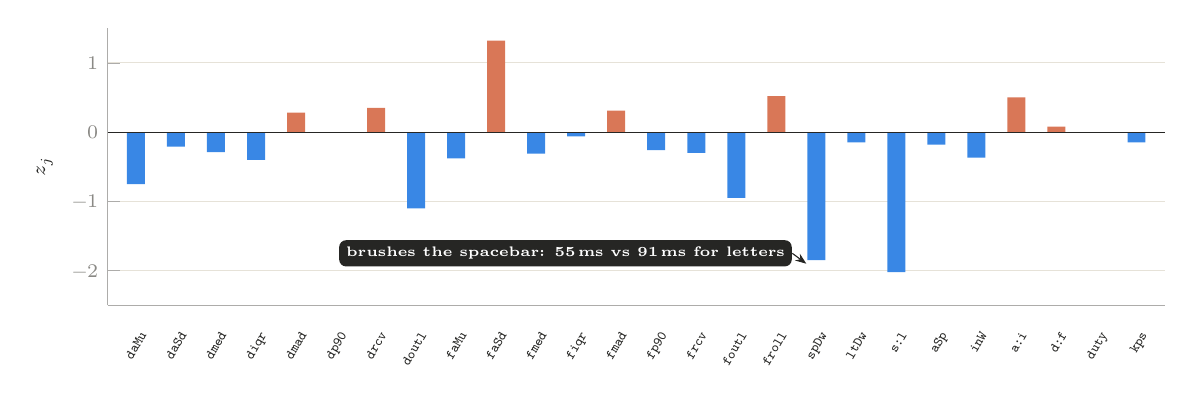
\begin{tikzpicture}
\begin{axis}[kl, ybar, bar width=6.5pt, width=15cm, height=5.1cm, ymin=-2.5, ymax=1.5,
    xmin=-0.7, xmax=25.7, enlarge x limits=false, ymajorgrids, ylabel={\(z_j\)},
    xtick={0,...,25}, major x tick style={draw=none},
    xticklabels={daMu,daSd,dmed,diqr,dmad,dp90,drcv,doutl,faMu,faSd,fmed,fiqr,fmad,fp90,frcv,foutl,froll,spDw,ltDw,s:l,aSp,inW,a:i,d:f,duty,kps},
    xticklabel style={rotate=60, anchor=north east, font=\ttfamily\tiny, text=ink}, clip=false]
  \addplot[fill=terra, draw=none, bar shift=0pt] coordinates {(4,0.28) (6,0.35) (9,1.32) (12,0.31) (16,0.52) (22,0.50) (23,0.08)};
  \addplot[fill=sky, draw=none, bar shift=0pt] coordinates {(0,-0.75) (1,-0.21) (2,-0.29) (3,-0.40) (7,-1.10) (8,-0.38) (10,-0.31) (11,-0.06) (13,-0.26) (14,-0.30) (15,-0.95) (17,-1.85) (18,-0.15) (19,-2.02) (20,-0.18) (21,-0.37) (25,-0.15)};
  \draw[ink] (axis cs:-0.7,0) -- (axis cs:25.7,0);
  \node[pill=ink,anchor=east] (n) at (axis cs:16.4,-1.75) {brushes the spacebar: 55\,ms vs 91\,ms for letters};
  \draw[ink,-{Stealth[length=4pt]}] (n.east) -- (axis cs:16.75,-1.9);
\end{axis}
\end{tikzpicture}

\vspace{1mm}
\begin{columns}[T,onlytextwidth]
\column{0.4\textwidth}
\[ z_j = \frac{x_j - \mu_j}{\sigma_j}, \qquad \sigma_j \leftarrow \max(\sigma_j, 10^{-8}) \]
\column{0.57\textwidth}
\scriptsize Feature scales differ wildly (ratios \(\sim\)0--1, timings \(\sim\)0.02--0.3\,s, kps \(\sim\)2--8), so every
distance works in z-space. The \code{ZScoreScaler} is \textbf{fit on the training / enrolled data only}. In leave-one-out
evaluation it is re-fit for every fold, so no test statistic leaks in. \textcolor{terra}{\(\blacksquare\)} above the population mean,
\textcolor{sky}{\(\blacksquare\)} below.
\end{columns}
\end{frame}

% -----------------------------------------------------------------------------
\begin{frame}{Step 7 \textperiodcentered\ Templates: a point \emph{plus} a spread}
\begin{columns}[c,onlytextwidth]
\column{0.5\textwidth}
\centering
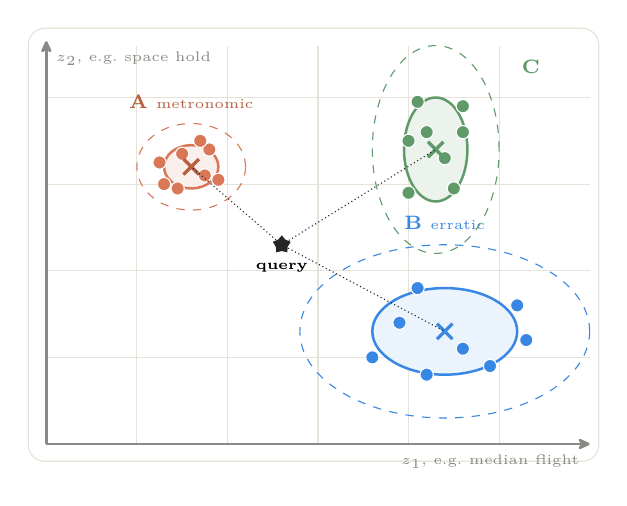
\begin{tikzpicture}[x=1.15cm,y=1.1cm]
  \fill[white,rounded corners=6pt,draw=line] (-0.2,-0.2) rectangle (6.1,4.8);
  \foreach \x in {1,2,...,5} \draw[line] (\x,0) -- (\x,4.6);
  \foreach \y in {1,2,...,4} \draw[line] (0,\y) -- (6,\y);
  \draw[flow] (0,0) -- (6.0,0) node[below left,font=\tiny,text=muted] {\(z_1\), e.g.\ median flight};
  \draw[flow] (0,0) -- (0,4.65) node[below right,font=\tiny,text=muted] {\(z_2\), e.g.\ space hold};
  % user A: metronomic
  \draw[terra,line width=0.9pt,fill=terra!12] (1.6,3.2) ellipse (0.3 and 0.25);
  \draw[terra,dashed] (1.6,3.2) ellipse (0.6 and 0.5);
  \foreach \p in {(1.3,3.0),(1.8,3.4),(1.5,3.35),(1.9,3.05),(1.45,2.95),(1.7,3.5),(1.25,3.25),(1.75,3.1)} \node[pt=terra] at \p {};
  \node[font=\scriptsize\bfseries,text=terradk] at (1.6,3.95) {A \textmd{\tiny metronomic}};
  % user B: erratic
  \draw[sky,line width=0.9pt,fill=sky!10] (4.4,1.3) ellipse (0.8 and 0.5);
  \draw[sky,dashed] (4.4,1.3) ellipse (1.6 and 1.0);
  \foreach \p in {(3.6,1.0),(5.2,1.6),(4.1,1.8),(4.9,0.9),(3.9,1.4),(4.6,1.1),(5.3,1.2),(4.2,0.8)} \node[pt=sky] at \p {};
  \node[font=\scriptsize\bfseries,text=sky] at (4.4,2.55) {B \textmd{\tiny erratic}};
  % user C
  \draw[sage,line width=0.9pt,fill=sage!12] (4.3,3.4) ellipse (0.35 and 0.6);
  \draw[sage,dashed] (4.3,3.4) ellipse (0.7 and 1.2);
  \foreach \p in {(4.0,2.9),(4.6,3.9),(4.2,3.6),(4.5,2.95),(4.1,3.95),(4.4,3.3),(4.0,3.5),(4.6,3.6)} \node[pt=sage] at \p {};
  \node[font=\scriptsize\bfseries,text=sage] at (5.35,4.35) {C};
  % centres
  \foreach \p/\c in {(1.6,3.2)/terradk,(4.4,1.3)/sky,(4.3,3.4)/sage} \node[cross out,draw=\c,line width=1.2pt,inner sep=2.2pt] at \p {};
  % query
  \node[star,star points=5,fill=ink,inner sep=1.6pt] (q) at (2.6,2.3) {};
  \foreach \p in {(1.6,3.2),(4.4,1.3),(4.3,3.4)} \draw[ink,densely dotted] (q) -- \p;
  \node[font=\tiny\bfseries,anchor=north] at (2.6,2.2) {query};
\end{tikzpicture}

{\scriptsize\color{muted}\(\times\) template mean \quad solid / dashed: 1\(\sigma\) / 2\(\sigma\) spread}

\column{0.47\textwidth}
\begin{card}[terra]{\ttfamily Template(user\_id, mean, std, n)}
\scriptsize
\(\mu_u = \operatorname{mean}\{\, z_i : y_i = u \,\}\)\\[4pt]
\(\sigma_u = \max\!\big(\operatorname{std}\{ z_i : y_i = u \},\ 0.25\,\sigma_{\text{pop}} + 10^{-6}\big)\)\\[3pt]
{\scriptsize per feature, in z-space, by \code{build\_templates}.}
\end{card}
\begin{card}[amber]{\faIcon{shield-alt}\ The spread floor}
\scriptsize Enrolled from two samples, a user can show near-zero spread on a feature \emph{purely by luck}; dividing by it
would let one coincidence outweigh everything. So spread never drops below 25\,\% of the population's (\code{SPREAD\_FLOOR}).
\end{card}
\end{columns}
\end{frame}

% -----------------------------------------------------------------------------
\begin{frame}{Step 8 \textperiodcentered\ Distance: scaled Manhattan}
\vspace{2mm}
\begin{columns}[c,onlytextwidth]
\column{0.5\textwidth}
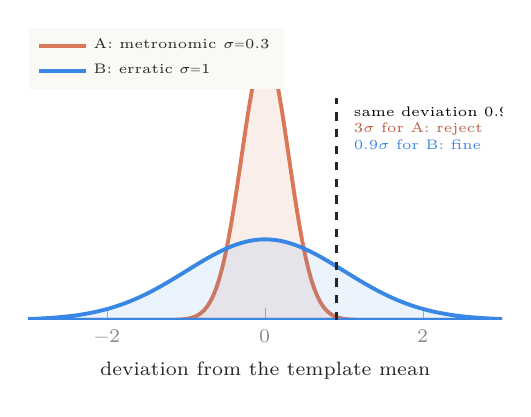
\begin{tikzpicture}
\begin{axis}[kl, width=7.6cm, height=5.3cm, xmin=-3, xmax=3, ymin=0, ymax=1.45, samples=160,
   ytick=\empty, xlabel={deviation from the template mean}, axis x line*=bottom, axis y line=none,
   legend style={at={(0.0,1.0)},anchor=north west,font=\tiny,fill=paper}]
  \addplot[terra, line width=1.4pt, fill=terra, fill opacity=0.12, domain=-3:3] {exp(-x^2/(2*0.09))/(0.3*sqrt(2*pi))} \closedcycle;
  \addplot[sky, line width=1.4pt, fill=sky, fill opacity=0.10, domain=-3:3] {exp(-x^2/2)/sqrt(2*pi)} \closedcycle;
  \legend{A: metronomic \(\sigma{=}0.3\), B: erratic \(\sigma{=}1\)}
  \draw[ink,dashed,line width=0.9pt] (axis cs:0.9,0) -- (axis cs:0.9,1.1);
  \node[font=\tiny,anchor=west,align=left] at (axis cs:1.0,0.95) {same deviation 0.9:\\\textcolor{terradk}{3\(\sigma\) for A: reject}\\\textcolor{sky}{0.9\(\sigma\) for B: fine}};
\end{axis}
\end{tikzpicture}

\column{0.47\textwidth}
\begin{tcolorbox}[enhanced,colback=white,colframe=terra!45,boxrule=0.6pt,arc=6pt,halign=center,top=3pt,bottom=3pt,
  before skip=0pt,after skip=6pt,fuzzy shadow={0.4pt}{-0.9pt}{0pt}{0.35pt}{black!10}]
\(\displaystyle D(q,u) \;=\; \frac{1}{26}\sum_{j=1}^{26} \frac{\big|\,q_j - \mu_{u,j}\,\big|}{\sigma_{u,j}}\)
\end{tcolorbox}
\begin{card}[terra]{\faBalanceScale\ Divide by \emph{that user's} spread}
\scriptsize Rejects a metronomic typist for a slip that is normal for an erratic one; a population z-score can't.
\textbf{EER 7.98\,\% \(\rightarrow\) 5.45\,\%}: the biggest single win in the decision layer.
\end{card}
\begin{card}[sky]{\faRulerCombined\ Manhattan, not Euclidean}
\scriptsize Squaring lets one wildly-off feature dominate; absolute deviations let the other 25 outvote it.
\end{card}
\end{columns}
\end{frame}

% -----------------------------------------------------------------------------
\begin{frame}{Step 9 \textperiodcentered\ Identification: distance-weighted \(k\)-NN}
\begin{columns}[c,onlytextwidth]
\column{0.45\textwidth}
\centering
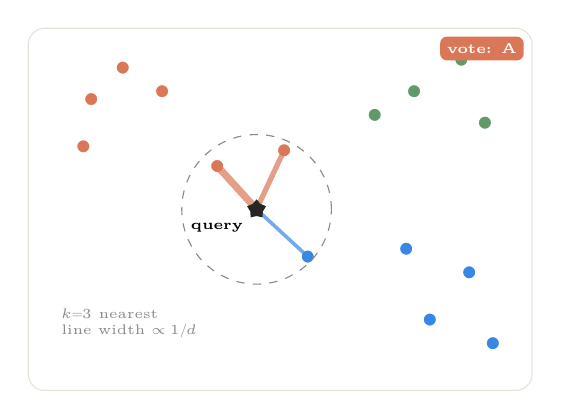
\begin{tikzpicture}[x=1cm,y=1cm]
  \fill[white,rounded corners=6pt,draw=line] (-0.3,-0.3) rectangle (6.1,4.3);
  \foreach \p in {(0.5,3.4),(0.9,3.8),(0.4,2.8),(1.4,3.5),(2.1,2.55),(2.95,2.75)} \node[pt=terra] at \p {};
  \foreach \p in {(4.8,0.6),(5.3,1.2),(4.5,1.5),(3.25,1.4),(5.6,0.3)} \node[pt=sky] at \p {};
  \foreach \p in {(4.6,3.5),(5.2,3.9),(5.5,3.1),(4.1,3.2)} \node[pt=sage] at \p {};
  \coordinate (q) at (2.6,2.0);
  \draw[muted,dashed] (q) circle (0.95);
  \draw[terra,line width=2.6pt,line cap=round,opacity=0.7] (q) -- (2.1,2.55);
  \draw[terra,line width=1.9pt,line cap=round,opacity=0.7] (q) -- (2.95,2.75);
  \draw[sky,line width=1.3pt,line cap=round,opacity=0.7] (q) -- (3.25,1.4);
  \node[star,star points=5,fill=ink,inner sep=1.7pt] at (q) {};
  \node[font=\tiny\bfseries,anchor=north east] at (2.55,1.95) {query};
  \node[font=\tiny,text=muted,anchor=west,align=left] at (0.0,0.55) {\(k{=}3\) nearest\\line width \(\propto 1/d\)};
  \node[pill=terra,anchor=north east] at (6.0,4.2) {vote: A};
\end{tikzpicture}

\column{0.52\textwidth}
\begin{card}[terra]{The vote}
\small
\(d_i = \sum_j |q_j - x_{ij}|\) \hfill{\scriptsize\color{muted}sample to sample, in z-space}\\[5pt]
\(\operatorname{score}(u) = \displaystyle\sum_{i \in \mathcal{N}_3(q),\ y_i = u} \frac{1}{d_i + 10^{-9}}\)\\[4pt]
\(\hat y = \arg\max_u \operatorname{score}(u)\)\\[3pt]
\scriptsize A near-identical neighbour outweighs one that just scraped into the top \(k\), and there is no arbitrary tie-break when \(k\) splits evenly.
\end{card}
\begin{card}[sky]{\faIcon{sync-alt}\ Leave-one-out cross-validation}
\scriptsize For each of the 48 real samples: refit the scaler on the other 47, predict it. \textbf{38 / 48 = 79.2\,\%}
across 6 typists (chance \(\approx\) 17\,\%).
\end{card}
\end{columns}
\end{frame}

% -----------------------------------------------------------------------------
\begin{frame}{Step 10 \textperiodcentered\ Verification: genuine vs impostor}
\begin{columns}[c,onlytextwidth]
\column{0.58\textwidth}
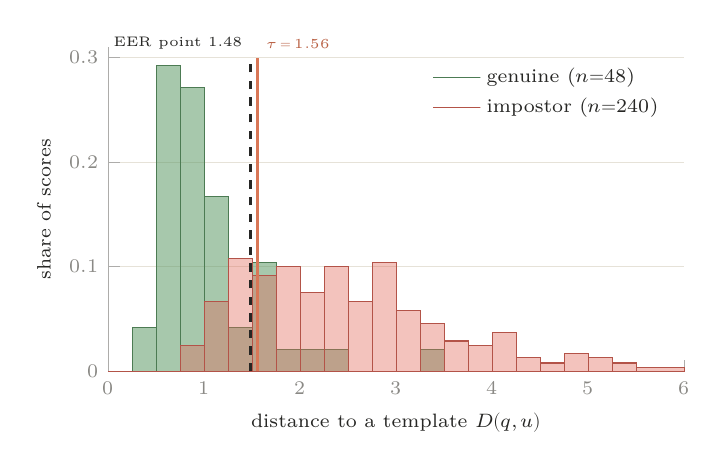
\begin{tikzpicture}
\begin{axis}[kl, width=8.9cm, height=5.7cm, xmin=0, xmax=6, ymin=0, ymax=0.31,
   xlabel={distance to a template \(D(q,u)\)}, ylabel={share of scores}, ymajorgrids,
   legend style={at={(0.98,0.97)},anchor=north east}, clip=false]
  \addplot[ybar interval, fill=sage, fill opacity=0.55, draw=sage!80!black] coordinates {(0.00,0.000) (0.25,0.042) (0.50,0.292) (0.75,0.271) (1.00,0.167) (1.25,0.042) (1.50,0.104) (1.75,0.021) (2.00,0.021) (2.25,0.021) (2.50,0) (2.75,0) (3.00,0) (3.25,0.021) (3.50,0) (6.0,0)};
  \addplot[ybar interval, fill=rose, fill opacity=0.40, draw=rose!80!black] coordinates {(0.00,0.000) (0.25,0.000) (0.50,0.000) (0.75,0.025) (1.00,0.067) (1.25,0.108) (1.50,0.092) (1.75,0.100) (2.00,0.075) (2.25,0.100) (2.50,0.067) (2.75,0.104) (3.00,0.058) (3.25,0.046) (3.50,0.029) (3.75,0.025) (4.00,0.037) (4.25,0.013) (4.50,0.008) (4.75,0.017) (5.00,0.013) (5.25,0.008) (5.50,0.004) (6.0,0)};
  \legend{genuine (\(n{=}48\)), impostor (\(n{=}240\))}
  \draw[ink,dashed,line width=0.9pt] (axis cs:1.483,0) -- (axis cs:1.483,0.30) node[above left=-1pt,font=\tiny] {EER point 1.48};
  \draw[terra,line width=1.1pt] (axis cs:1.557,0) -- (axis cs:1.557,0.30) node[above right=-1pt,font=\tiny\bfseries,text=terradk] {\(\tau = 1.56\)};
\end{axis}
\end{tikzpicture}

\column{0.39\textwidth}
\begin{card}[sage]{Protocol (\code{verification\_scores})}
\scriptsize For every sample \(i\):
\begin{enumerate}\setlength\itemsep{1pt}
\item refit the scaler \emph{without} \(i\)
\item build all templates from the rest
\item \textbf{genuine}: \(D(x_i, \text{own template})\)
\item \textbf{impostor}: \(D(x_i, \text{every other})\)
\end{enumerate}
\end{card}
{\small Genuine mean \textbf{1.04}\,\textcolor{muted}{(sd 0.56)}\\ Impostor mean \textbf{2.48}\,\textcolor{muted}{(sd 1.06)}}\\[2pt]
{\scriptsize\color{muted}Real captures, 6 users. The overlap of the two humps is the error we trade.}
\end{columns}
\end{frame}

% -----------------------------------------------------------------------------
\begin{frame}{Step 11 \textperiodcentered\ Equal error rate and operating point}
\begin{columns}[c,onlytextwidth]
\column{0.56\textwidth}
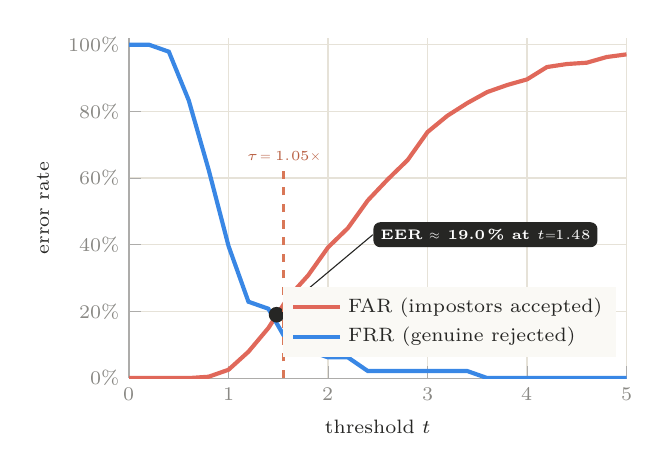
\begin{tikzpicture}
\begin{axis}[kl, width=7.9cm, height=5.9cm, xmin=0, xmax=5, ymin=0, ymax=1.02,
   xlabel={threshold \(t\)}, ylabel={error rate}, ymajorgrids, xmajorgrids,
   legend style={at={(0.98,0.06)},anchor=south east,fill=paper}, yticklabel={\pgfmathparse{\tick*100}\pgfmathprintnumber[fixed,precision=0]{\pgfmathresult}\%}]
  \addplot[rose, line width=1.5pt, mark=none] coordinates {(0.00,0.000) (0.20,0.000) (0.40,0.000) (0.60,0.000) (0.80,0.004) (1.00,0.025) (1.20,0.079) (1.40,0.150) (1.60,0.242) (1.80,0.308) (2.00,0.392) (2.20,0.450) (2.40,0.533) (2.60,0.596) (2.80,0.654) (3.00,0.738) (3.20,0.787) (3.40,0.825) (3.60,0.858) (3.80,0.879) (4.00,0.896) (4.20,0.933) (4.40,0.942) (4.60,0.946) (4.80,0.963) (5.00,0.971)};
  \addplot[sky, line width=1.5pt, mark=none] coordinates {(0.00,1.000) (0.20,1.000) (0.40,0.979) (0.60,0.833) (0.80,0.625) (1.00,0.396) (1.20,0.229) (1.40,0.208) (1.60,0.104) (1.80,0.083) (2.00,0.062) (2.20,0.062) (2.40,0.021) (2.60,0.021) (2.80,0.021) (3.00,0.021) (3.20,0.021) (3.40,0.021) (3.60,0.000) (3.80,0.000) (4.00,0.000) (4.20,0.000) (4.40,0.000) (4.60,0.000) (4.80,0.000) (5.00,0.000)};
  \legend{FAR (impostors accepted), FRR (genuine rejected)}
  \node[circle,fill=ink,inner sep=2pt] at (axis cs:1.483,0.190) {};
  \node[pill=ink,anchor=west] (eer) at (axis cs:2.45,0.43) {EER \(\approx\) 19.0\,\% at \(t{=}1.48\)};
  \draw[ink,-{Stealth[length=4pt]}] (eer.west) -- (axis cs:1.53,0.20);
  \draw[terra,line width=1.1pt,dashed] (axis cs:1.557,0) -- (axis cs:1.557,0.62) node[above,font=\tiny\bfseries,text=terradk] {\(\tau = 1.05\times\)};
\end{axis}
\end{tikzpicture}

\column{0.41\textwidth}
\scriptsize
\(\mathrm{FAR}(t)=\Pr[D_{\text{imp}}\le t]\),\quad \(\mathrm{FRR}(t)=\Pr[D_{\text{gen}}>t]\).
Sweep 500 thresholds; the EER is where \(|\mathrm{FAR}-\mathrm{FRR}|\) is smallest.

\vspace{1.5mm}
\renewcommand\arraystretch{1.15}
\arrayrulecolor{line}
\setlength\tabcolsep{4pt}
\begin{tabular}{@{}c r r r@{}}
\rowcolor{ink}\textcolor{cream}{\bfseries \(\tau\) / \(t_{\text{EER}}\)} & \textcolor{cream}{rejected} & \textcolor{cream}{accepted} & \textcolor{cream}{\bfseries HTER}\\
\(\times\)1.00 & 5.8\,\% & 6.1\,\% & 5.95\,\% \\ \midrule
\rowcolor{terra!12}\(\times\)\textbf{1.05} & \textbf{5.0\,\%} & \textbf{7.3\,\%} & \textbf{6.13\,\%} \\ \midrule
\(\times\)1.20 {\tiny\color{muted}old} & 2.5\,\% & 11.7\,\% & 7.11\,\% \\ \midrule
\(\times\)1.30 & 0.8\,\% & 14.5\,\% & 7.68\,\% \\
\end{tabular}

{\tiny\color{muted}cross-phrase benchmark, 8 users. HTER \(=\) (FAR \(+\) FRR) / 2.}

\vspace{1.5mm}
\code{ACCEPT\_TOLERANCE} \(=1.05\): the fewest total mistakes (exact optimum \(1.06\times\)). On real data it also
beats \(1.2\): 17.3\,\% vs 19.0\,\% HTER. \textbf{\(\tau\) decides \emph{whether} to answer, never \emph{who}.}
\end{columns}
\end{frame}

% -----------------------------------------------------------------------------
\begin{frame}{Step 12 \textperiodcentered\ Fusing a whole run into one verdict}
\begin{columns}[c,onlytextwidth]
\column{0.53\textwidth}
\centering
\scriptsize
\renewcommand\arraystretch{1.06}
\arrayrulecolor{line}
\begin{tabular}{@{}l c c c l@{}}
\rowcolor{ink}\textcolor{cream}{\bfseries sample} & \textcolor{cream}{\bfseries A} & \textcolor{cream}{\bfseries B} & \textcolor{cream}{\bfseries C} & \textcolor{cream}{per-sample vote}\\
\(s_1\) & \cellcolor{sage!20}0.80 & 1.90 & 1.40 & A \\ \midrule
\rowcolor{rose!8}\(s_2\) \textcolor{rose}{\faBell} & 1.70 & \cellcolor{rose!25}1.50 & 2.20 & \textcolor{rose}{\textbf{B} \faTimes}\\ \midrule
\(s_3\) & \cellcolor{sage!20}0.90 & 2.10 & 1.60 & A \\ \midrule
\(s_4\) & \cellcolor{sage!20}1.00 & 1.80 & 1.30 & A \\ \midrule
\(s_5\) & \cellcolor{sage!20}0.70 & 2.00 & 1.50 & A \\ \midrule
\rowcolor{terra!14}\textbf{mean} & \textbf{1.02} & 1.86 & 1.60 & \(\Rightarrow\) \textbf{A}, margin 0.58\\
\end{tabular}

\vspace{1mm}
{\tiny\color{muted}illustrative numbers; \(s_2\): a phone buzzed mid-sentence.}

\vspace{1.5mm}
\begin{card}[terra]{\code{fuse()}: pool distances, not votes}
\scriptsize One run's samples are \emph{known} to share a typist. Averaging distances keeps a second-best sample's evidence;
a vote throws it away. Mean beat median and min pooling.
\end{card}

\column{0.44\textwidth}
\centering
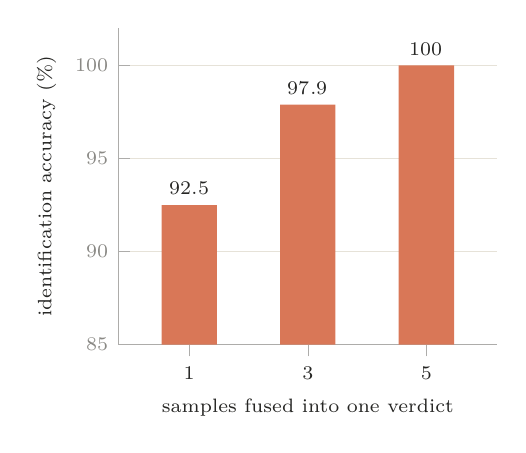
\begin{tikzpicture}
\begin{axis}[kl, ybar, bar width=20pt, width=6.4cm, height=5.6cm, ymin=85, ymax=102,
    symbolic x coords={1,3,5}, xtick=data, ymajorgrids, enlarge x limits=0.3,
    xlabel={samples fused into one verdict}, ylabel={identification accuracy (\%)},
    nodes near coords, every node near coord/.append style={font=\scriptsize\bfseries,text=ink},
    x tick label style={font=\scriptsize,text=ink}]
  \addplot[fill=terra, draw=none] coordinates {(1,92.5) (3,97.9) (5,100)};
\end{axis}
\end{tikzpicture}

{\scriptsize\color{muted}cross-phrase benchmark, leave-one-phrase-out}
\end{columns}
\end{frame}

% -----------------------------------------------------------------------------
\begin{frame}{The decision, end to end}
\centering
\begin{tikzpicture}[yscale=0.88]
  \node[box=ink,fill=ink!6] (fin) at (0,0) {\faFlagCheckered\ typing test finished\\run \(\rightarrow\) samples};
  \node[dec=amber] (enough) at (3.7,0) {\(\ge\)1 sample\\of 16+ keys?};
  \node[box=rose] (short) at (3.7,-2.2) {“too short, keep typing”\\new test dealt};
  \node[box=sky] (feat) at (7.4,0) {26-D vector per sample\\\code{identify()}: kNN vote + all \(D(q,u)\)};
  \node[box=terra] (fuse) at (11.1,0) {\code{fuse()}\\mean \(D\) per user, ranked};
  \node[dec=sage] (thr) at (11.1,-2.2) {\(D_{\min} \le \tau\)?};
  \node[box=sage,fill=sage!22,line width=1.1pt] (ok) at (11.1,-4.25) {\faTrophy\ \textbf{name} typed out\\closest template + margin};
  \node[box=rose] (un) at (7.4,-2.2) {\textsc{unrecognized}\\“type again”: fresh test};
  \node[box=muted,fill=white,text width=3.9cm,align=left] (conf) at (6.6,-4.25)
    {\textbf{confidence} from the margin to 2nd place:\\ \(>1.0\) \textcolor{sage}{high} \enspace \(>0.4\) \textcolor{amber!85!black}{moderate} \enspace else \textcolor{rose}{low}};

  \draw[flow] (fin) -- (enough);
  \draw[flow] (enough) -- node[above,dlab=sage] {yes} (feat);
  \draw[flow] (enough) -- node[right,dlab=rose] {no} (short);
  \draw[flow] (feat) -- (fuse);
  \draw[flow] (fuse) -- (thr);
  \draw[flow] (thr) -- node[right,dlab=sage] {yes} (ok);
  \draw[flow] (thr) -- node[above,dlab=rose] {no} (un);
  \draw[flow,dashed,rose!70] (un.south) -- ++(0,-0.35) -| ($(fin.south)+(0.35,0)$);
  \draw[flow,dashed,rose!70] (short.west) -| ($(fin.south)+(-0.35,0)$);
  \node[font=\tiny,text=rose!80!black,anchor=north] at (2.2,-3.45) {keep typing: a fresh test is dealt};
  \draw[muted,dotted,line width=0.9pt] (conf.east) -- (ok.west);
\end{tikzpicture}

\vspace{0.5mm}
{\scriptsize\color{muted}Heavy work (enrolled matrix, EER sweep, identification) runs on a worker thread; the UI polls the result queue every 120\,ms and never blocks.}
\end{frame}

% -----------------------------------------------------------------------------
\begin{frame}{A real identification, bar by bar}
\begin{columns}[c,onlytextwidth]
\column{0.58\textwidth}
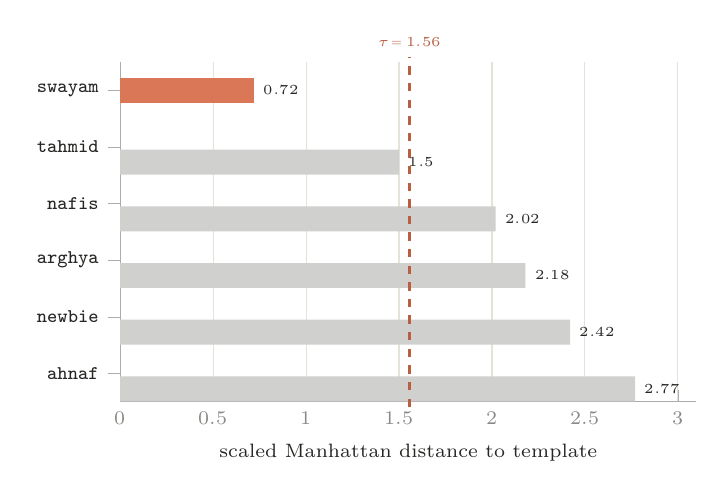
\begin{tikzpicture}
\begin{axis}[kl, xbar, bar width=9pt, width=8.9cm, height=5.9cm, xmin=0, xmax=3.1,
    symbolic y coords={ahnaf,newbie,arghya,nafis,tahmid,swayam}, ytick={ahnaf,newbie,arghya,nafis,tahmid,swayam}, y dir=normal,
    xlabel={scaled Manhattan distance to template}, xmajorgrids, enlarge y limits=0.1,
    yticklabel style={font=\ttfamily\scriptsize,text=ink},
    nodes near coords, every node near coord/.append style={font=\tiny,text=ink}, clip=false]
  \addplot[fill=muted!40, draw=none] coordinates {(2.77,ahnaf) (2.42,newbie) (2.18,arghya) (2.02,nafis) (1.50,tahmid)};
  \addplot[fill=terra, draw=none, bar shift=0pt] coordinates {(0.72,swayam)};
  \draw[terradk,dashed,line width=1pt] ([yshift=-12pt]axis cs:1.557,ahnaf) --([yshift=12pt]axis cs:1.557,swayam) node[above,font=\tiny\bfseries,text=terradk] {\(\tau=1.56\)};
\end{axis}
\end{tikzpicture}

\column{0.39\textwidth}
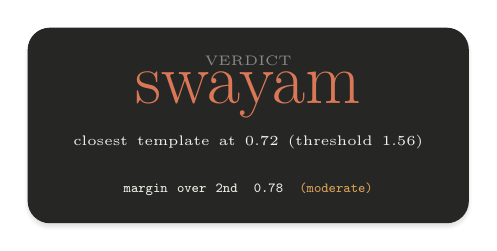
\begin{tikzpicture}
  \node[fill=ink,rounded corners=8pt,text width=4.9cm,inner sep=10pt,align=center,soft shadow] {
    {\tiny\color{muted}VERDICT}\\[2pt]
    {\titlefont\fontsize{26}{28}\selectfont\color{terra}swayam}\\[3pt]
    {\tiny\color{cream!75}closest template at 0.72 (threshold 1.56)}\\[5pt]
    {\ttfamily\tiny\color{cream}margin over 2nd \enspace 0.78 \enspace\textcolor{amber}{(moderate)}}};
\end{tikzpicture}

\vspace{2mm}
\scriptsize One of \texttt{swayam}'s enrolled samples scored against all 6 templates. It is in-sample, so shown only to illustrate the mechanics.

\vspace{1mm}
The runner-up, \texttt{tahmid}, sits 0.78 further away: above 0.4 but under 1.0, so the verdict is reported with
\textcolor{amber!85!black}{\textbf{moderate confidence}}.
\end{columns}
\end{frame}

% -----------------------------------------------------------------------------
\begin{frame}{How we measured it}
\begin{columns}[T,onlytextwidth]
\column{0.44\textwidth}
{\small\bfseries Leave-one-\emph{phrase}-out}\par\vspace{1mm}
\centering
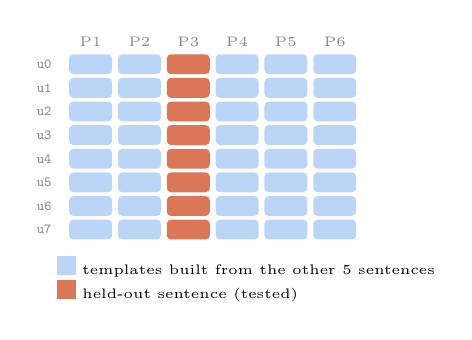
\begin{tikzpicture}[x=0.62cm,y=0.3cm]
  \foreach \u in {0,...,7} {
    \node[font=\tiny\ttfamily,text=muted,anchor=east] at (-0.1,-\u) {u\u};
    \foreach \p in {0,...,5} {
      \ifnum\p=2 \fill[terra,rounded corners=1.5pt] (\p+0.06,-\u-0.42) rectangle (\p+0.94,-\u+0.42);
      \else \fill[sky!35,rounded corners=1.5pt] (\p+0.06,-\u-0.42) rectangle (\p+0.94,-\u+0.42);\fi
    }}
  \foreach \p in {1,...,6} \node[font=\tiny,text=muted] at (\p-0.5,0.95) {P\p};
  \node[font=\tiny,anchor=north west,align=left] at (-0.4,-7.7) {\swatch{sky!35} templates built from the other 5 sentences\\\swatch{terra} held-out sentence (tested)};
\end{tikzpicture}
\raggedright
\vspace{1mm}

\scriptsize Leave-one-\emph{sample}-out would compare a sample with siblings from the same sentence, flattering features that
encode the sentence, not the typist.

\column{0.53\textwidth}
{\small\bfseries The fixture} {\scriptsize\code{tools/benchmark\_inference.py}}\par\vspace{1mm}
\scriptsize 8 simulated users \(\times\) 6 pangrams \(\times\) 5 repeats = \textbf{240 samples}; each user has a fixed profile:

\vspace{1mm}
\renewcommand\arraystretch{1.04}
\setlength\tabcolsep{4pt}
\arrayrulecolor{line}
\begin{tabular}{@{}l l@{}}
\rowcolor{ink}\textcolor{cream}{\bfseries parameter} & \textcolor{cream}{\bfseries distribution}\\
dwell (mean / sd)     & \(\mathcal U(70,160)\) / \(\mathcal U(10,30)\) ms \\ \midrule
flight (mean / sd)    & \(\mathcal U(80,300)\) / \(\mathcal U(20,60)\) ms \\ \midrule
per-key bias          & \(\times\,\mathcal U(0.8,1.3)\), fixed per key \\ \midrule
\rowcolor{terra!8} rollover & \(p\sim\mathcal U(.03,.22)\); gap \(=-\mathcal U(.005,.6)\,\times\) hold \\ \midrule
\rowcolor{terra!8} think-pause & \(p\sim\mathcal U(.01,.06)\); gap \(+\mathrm{Exp}(\mathcal U(.15,.6)\,\text{s})\) \\
\end{tabular}

\vspace{1.5mm}
\begin{card}[terra]{Why add keyboard realism?}
\scriptsize The plain generator clamps flights at \(+10\) ms, so it never produces rollover (12.8\,\% in the fixture, 16.0\,\% in real captures).
\end{card}
\end{columns}
\end{frame}

% -----------------------------------------------------------------------------
\begin{frame}{Results}
\begin{columns}[c,onlytextwidth]
\column{0.53\textwidth}
\scriptsize
\renewcommand\arraystretch{1.3}
\arrayrulecolor{line}
\begin{tabular}{@{}l l c r r r r@{}}
\rowcolor{ink}
\textcolor{cream}{\bfseries set} & \textcolor{cream}{\bfseries vector} & \textcolor{cream}{dim} & \textcolor{cream}{1 smp} & \textcolor{cream}{fuse 3} & \textcolor{cream}{fuse 5} & \textcolor{cream}{EER}\\
fixture & spectral & 14 & 68.8 & 72.9 & 72.9 & 18.72 \\ \midrule
\rowcolor{terra!12}
fixture & \textbf{timing} & 26 & \textbf{92.5} & \textbf{97.9} & \textbf{100.0} & \textbf{5.89} \\ \midrule
real    & spectral & 14 & 56.2 & n/a & n/a & 29.79 \\ \midrule
\rowcolor{terra!12}
real    & \textbf{timing} & 26 & \textbf{79.2} & n/a & n/a & \textbf{18.96} \\
\end{tabular}

\vspace{2mm}
{\color{muted}All in \%. Fixture: 240 samples, 8 users, leave-one-phrase-out. Real: 48 samples, 6 users, one session each,
so only leave-one-sample-out is possible and runs are too short to fuse.}

\vspace{2mm}
\begin{card}[sky]{Reading it}
\scriptsize The timing vector wins everywhere. Real data is harder: one session per typist, and \texttt{newbie} enrolled only 3 samples.
\end{card}

\column{0.44\textwidth}
\centering
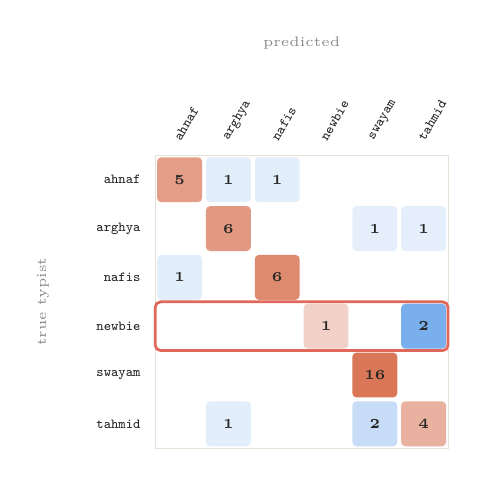
\begin{tikzpicture}[x=0.62cm,y=0.62cm]
  \def\names{{"ahnaf","arghya","nafis","newbie","swayam","tahmid"}}
  \foreach \r/\row/\tot in {0/{5,1,1,0,0,0}/7, 1/{0,6,0,0,1,1}/8, 2/{1,0,6,0,0,0}/7,
                            3/{0,0,0,1,0,2}/3, 4/{0,0,0,0,16,0}/16, 5/{0,1,0,0,2,4}/7} {
    \foreach \v [count=\c from 0] in \row {
      \pgfmathtruncatemacro\shade{round(100*\v/\tot)}
      \ifnum\c=\r \fill[terra!\shade!white,rounded corners=1.5pt] (\c+0.04,-\r-0.96) rectangle (\c+0.96,-\r-0.04);
      \else \fill[sky!\shade!white,rounded corners=1.5pt] (\c+0.04,-\r-0.96) rectangle (\c+0.96,-\r-0.04);\fi
      \ifnum\v>0 \node[font=\tiny\bfseries,text=ink] at (\c+0.5,-\r-0.5) {\v};\fi
    }
    \pgfmathsetmacro\nm{\names[\r]}
    \node[font=\tiny\ttfamily,anchor=east,text=ink] at (-0.1,-\r-0.5) {\nm};
    \node[font=\tiny\ttfamily,anchor=west,rotate=60,text=ink] at (\r+0.35,0.15) {\nm};
  }
  \draw[line] (0,0) rectangle (6,-6);
  \node[font=\tiny,text=muted,rotate=90] at (-2.3,-3) {true typist};
  \node[font=\tiny,text=muted] at (3,2.3) {predicted};
  \draw[rose,line width=1pt,rounded corners=2pt] (0,-3) rectangle (6,-4);
\end{tikzpicture}

{\scriptsize\color{muted}Real captures, LOOCV \(k\)-NN: 38 / 48. \textcolor{rose}{Row}: \texttt{newbie}, only 3 samples to learn from.}
\end{columns}
\end{frame}

% -----------------------------------------------------------------------------
\begin{frame}{Engineering the app}
\begin{columns}[T,onlytextwidth]
\column{0.55\textwidth}
\centering
\begin{tikzpicture}
  \node[elane=sky] (ui) at (0,0) {};
  \node[elane=terra] (wk) at (4.6,0) {};
  \node[font=\scriptsize\bfseries,text=sky,anchor=north] at (ui.north) {\faDesktop\ Tk main thread};
  \node[font=\scriptsize\bfseries,text=terradk,anchor=north] at (wk.north) {\faCogs\ worker thread};
  \node[job=sky] at (0,1.25)  {key handlers \(\rightarrow\) \texttt{perf\_counter}};
  \node[job=sky] at (0,0.45)  {\texttt{Animator}: one 60\,fps tick for every tween};
  \node[job=sky] at (0,-0.35) {verdict, bars, charts};
  \node[job=sky] at (0,-1.15) {\texttt{\_poll\_worker} every 120\,ms};
  \node[job=terra] at (4.6,1.25)  {\texttt{build\_dataset}};
  \node[job=terra] at (4.6,0.45)  {EER threshold sweep};
  \node[job=terra] at (4.6,-0.35) {\texttt{identify} + \texttt{fuse}};
  \node[job=terra] at (4.6,-1.15) {explain: \texttt{build\_phases}};
  \draw[flow,terra] (1.65,0.9) -- node[above,font=\tiny,text=muted] {jobs} (2.95,0.9);
  \draw[flow,sky] (2.95,-0.75) -- node[below,font=\tiny,text=muted] {queue} (1.65,-0.75);
\end{tikzpicture}

\vspace{1mm}
\begin{card}[amber]{\faRocket\ The splash is not just a curtain}
\scriptsize A worker imports numpy + the pipeline and builds the enrolled matrix and EER threshold, so identify is warm on open.
\end{card}

\column{0.42\textwidth}
{\small\bfseries\faIcon{stopwatch}\ Motion vs timing fidelity}\par\vspace{1mm}
\scriptsize Animations share the thread that timestamps keys. Measured on a synthetic 40\,/\,60\,ms cadence:

\vspace{1mm}
\renewcommand\arraystretch{1.12}
\arrayrulecolor{line}
\begin{tabular}{@{}l r r@{}}
\rowcolor{ink}\textcolor{cream}{\bfseries} & \textcolor{cream}{motion off} & \textcolor{cream}{motion on}\\
flight sd       & 0.25 ms & 0.3 ms \\ \midrule
dwell jitter    & baseline & \(+\approx\)3 ms \\ \midrule
dwell worst     & baseline & \(\le\)16 ms \\ \midrule
handler bias    & \(\approx\)5 ms & \(\approx\)5 ms \\
\end{tabular}

\vspace{1.5mm}
Well inside human dwell variability (\(\sim\)10--30 ms). Cleanest enrollment:

\vspace{1mm}
\colorbox{ink}{\ttfamily\textcolor{cream}{KEYLOGGD\_NO\_ANIM=1 python main.py}}
\end{columns}
\end{frame}

% -----------------------------------------------------------------------------
\begin{frame}{Explain mode: the pipeline, one phase at a time}
\centering
\begin{tikzpicture}
  \phase{0}{terra}{\faKeyboard}{capture}{dwell \& flight per key}{grouped columns}
  \phase{1}{terra}{\faArrowsAltH}{zero-pad}{to \(N{=}32\)}{columns + shaded pad}
  \phase{2}{sky}{\faWaveSquare}{FFT}{\(|X[k]|\) per bin}{grouped columns}
  \phase{3}{sky}{\faTable}{features}{the 26 numbers}{a table (mixed units)}
  \phase{4}{amber}{\faSlidersH}{normalise}{z vs enrolled}{diverging columns}
  \phase{5}{sage}{\faBalanceScale}{decide}{\(D\) to every template}{bars + threshold}
  \foreach \a/\b in {0/1,1/2,2/3,3/4,4/5} \draw[flow] (p\a.east) -- (p\b.west);
\end{tikzpicture}

\vspace{2.5mm}
\begin{columns}[T,onlytextwidth]
\column{0.48\textwidth}
\begin{card}[terra]{\faCheckDouble\ Nothing re-implemented}
\scriptsize Each phase calls the \emph{same} functions the identify path calls and just keeps the intermediate values. If the
pipeline changes, the explainer changes with it instead of drifting into a pretty lie.
\end{card}
\column{0.48\textwidth}
\begin{card}[sky]{\faPlay\ Built to be presented}
\scriptsize A phase rail, the chart, and a values panel; step with next / previous or autoplay at 3.2\,s per phase.
Charts use a CVD-checked terracotta / blue pair on the dark panel.
\end{card}
\end{columns}
\end{frame}

% -----------------------------------------------------------------------------
\begin{frame}[fragile]{Running it}
\begin{columns}[T,onlytextwidth]
\column{0.6\textwidth}
\begin{tcolorbox}[enhanced,colback=ink,colframe=ink,arc=6pt,left=2pt,right=2pt,top=6pt,bottom=6pt,
  fuzzy shadow={0.4pt}{-0.9pt}{0pt}{0.35pt}{black!20}]
\begin{lstlisting}[style=shell]
pip install -r requirements.txt   # numpy>=2.4.2

python main.py                    # splash, then app
python main.py --no-splash
python main.py --data-dir DIR     # other enrolled set
KEYLOGGD_NO_ANIM=1 python main.py # cleanest timing

python -m keyloggd.ui.typing_test
python -m keyloggd.pipeline.classifier  # LOOCV + EER
python -m keyloggd.pipeline.identify_sample X.json
python -m tools.synthetic_data_generator
python -m tools.benchmark_inference [--real-only]
\end{lstlisting}
\end{tcolorbox}

\column{0.37\textwidth}
\small
\begin{itemize}\setlength\itemsep{4pt}
\item \textbf{Python 3 + tkinter + numpy}, nothing else. kNN, scaler, templates and the EER sweep are written from first principles.
\item \code{identify\_sample}: \code{--k}, \code{--threshold}, \code{--tolerance}, \code{--no-threshold}.
\item The benchmark re-checks every accuracy claim in the docstrings.
\end{itemize}
\end{columns}
\end{frame}

% -----------------------------------------------------------------------------
\begin{frame}{Takeaways \& what's next}
\begin{columns}[T,onlytextwidth]
\column{0.48\textwidth}
{\titlefont\large Takeaways}\par\vspace{2mm}
\small
\goodline{Typing rhythm identifies people: \textbf{92.5\,\%} from one 32-key sample, \textbf{100\,\%} with five, on the benchmark.}
\vspace{2pt}
\goodline{\textbf{Robust statistics} beat the spectrum for the decision; the spectrum still \emph{explains} rhythm best.}
\vspace{2pt}
\goodline{\textbf{Per-user spread} and \textbf{fusion} are the biggest wins of the decision layer.}
\vspace{2pt}
\goodline{A \textbf{game} gets natural typing and many samples, painlessly.}

\column{0.48\textwidth}
{\titlefont\large What's next}\par\vspace{2mm}
\begin{tikzpicture}
  \node[nx=terra] (a) at (0,0)     {\textbf{\faIcon{calendar-alt}\ More people, more days}: cross-session data to measure drift};
  \node[nx=sky]   (b) at (0,-0.95) {\textbf{\faIcon{sync-alt}\ Adaptive templates}: update slowly as someone's rhythm drifts};
  \node[nx=amber] (c) at (0,-1.9)  {\textbf{\faEye\ Continuous mode}: a background check after login};
  \node[nx=sage]  (d) at (0,-2.85) {\textbf{\faLock\ Protect the data}: encrypted templates, never raw logs};
  \node[nx=rose]  (e) at (0,-3.8)  {\textbf{\faUserSecret\ Liveness \& mimicry tests}: replay and trained-imitator attacks};
\end{tikzpicture}
\end{columns}
\end{frame}

% --------------------------------------------------------------- closing -----
{\setbeamercolor{background canvas}{bg=ink}
\begin{frame}[plain,noframenumbering]
\begin{tikzpicture}[remember picture,overlay]
  \coordinate (O) at (current page.south west);
  \foreach \x in {0,...,31} \foreach \y in {0,...,17}
    \fill[white,opacity=0.035] ($(O)+(0.25+\x*0.5,0.25+\y*0.5)$) circle (0.6pt);
  \node[anchor=west,text=cream,font=\titlefont\fontsize{44}{48}\selectfont] at ($(O)+(1.0,5.6)$) {Thank you};
  \node[anchor=west,text=muted,font=\large] at ($(O)+(1.05,4.45)$) {Questions? \enspace Or better: come and type.};
  \node[anchor=west,font=\ttfamily\large] at ($(O)+(1.05,3.35)$)
    {\textcolor{cream}{who is typi}\textcolor{terra}{\rule[-0.4ex]{1.6pt}{2.6ex}}\textcolor{muted}{ng right now}};
  \drawkeyboard{($(O)+(9.55,2.6)$)}
\end{tikzpicture}
\end{frame}}

\end{document}
